%%%%%%%%%%%%%%%%%%%%%%%%%%%%%%%%%%%%%%%%%
% The Legrand Orange Book
% LaTeX Template
% Version 2.1.1 (14/2/16)
%
% This template has been downloaded from:
% http://www.LaTeXTemplates.com
%
% Original author:
% Mathias Legrand (legrand.mathias@gmail.com) with modifications by:
% Vel (vel@latextemplates.com)
%
% License:
% CC BY-NC-SA 3.0 (http://creativecommons.org/licenses/by-nc-sa/3.0/)
%
% Compiling this template:
% This template uses biber for its bibliography and makeindex for its index.
% When you first open the template, compile it from the command line with the 
% commands below to make sure your LaTeX distribution is configured correctly:
%
% 1) pdflatex main
% 2) makeindex main.idx -s StyleInd.ist
% 3) biber main
% 4) pdflatex main x 2
%
% After this, when you wish to update the bibliography/index use the appropriate
% command above and make sure to compile with pdflatex several times 
% afterwards to propagate your changes to the document.
%
% This template also uses a number of packages which may need to be
% updated to the newest versions for the template to compile. It is strongly
% recommended you update your LaTeX distribution if you have any
% compilation errors.
%
% Important note:
% Chapter heading images should have a 2:1 width:height ratio,
% e.g. 920px width and 460px height.
%
%%%%%%%%%%%%%%%%%%%%%%%%%%%%%%%%%%%%%%%%%

%----------------------------------------------------------------------------------------
%	PACKAGES AND OTHER DOCUMENT CONFIGURATIONS
%----------------------------------------------------------------------------------------

\documentclass[10pt,fleqn,openany]{book} % Default font size and left-justified equations

%----------------------------------------------------------------------------------------

%%%%%%%%%%%%%%%%%%%%%%%%%%%%%%%%%%%%%%%%%
% The Legrand Orange Book
% Structural Definitions File
% Version 2.0 (9/2/15)
%
% Original author:
% Mathias Legrand (legrand.mathias@gmail.com) with modifications by:
% Vel (vel@latextemplates.com)
% 
% This file has been downloaded from:
% http://www.LaTeXTemplates.com
%
% License:
% CC BY-NC-SA 3.0 (http://creativecommons.org/licenses/by-nc-sa/3.0/)
%
%%%%%%%%%%%%%%%%%%%%%%%%%%%%%%%%%%%%%%%%%

%----------------------------------------------------------------------------------------
%	VARIOUS REQUIRED PACKAGES AND CONFIGURATIONS
%----------------------------------------------------------------------------------------

\usepackage[top=1cm,bottom=1cm,left=1cm,right=1cm,headsep=5pt,a5paper]{geometry} % Page margins

\usepackage{graphicx} % Required for including pictures
\graphicspath{{images/}} % Specifies the directory where pictures are stored

\usepackage{tikz} % Required for drawing custom shapes

\usepackage[english]{babel} % English language/hyphenation

\usepackage{enumitem} % Customize lists
\setlist{nolistsep} % Reduce spacing between bullet points and numbered lists

\usepackage{booktabs} % Required for nicer horizontal rules in tables

\usepackage{xcolor} % Required for specifying colors by name

\usepackage{multicol} % Required for multilines

\usepackage{pdflscape} % Required for landscape pages

\usepackage{wrapfig} % Required for wrapping text around figures

\definecolor{ocre}{RGB}{90,137,208} % Define the orange color used for highlighting throughout the book

%----------------------------------------------------------------------------------------
%	FONTS
%----------------------------------------------------------------------------------------

\usepackage{avant} % Use the Avantgarde font for headings
%\usepackage{times} % Use the Times font for headings
\usepackage{mathptmx} % Use the Adobe Times Roman as the default text font together with math symbols from the Sym­bol, Chancery and Com­puter Modern fonts

\usepackage{microtype} % Slightly tweak font spacing for aesthetics
\usepackage[utf8]{inputenc} % Required for including letters with accents
\usepackage[T1]{fontenc} % Use 8-bit encoding that has 256 glyphs

%----------------------------------------------------------------------------------------
%	BIBLIOGRAPHY AND INDEX
%----------------------------------------------------------------------------------------

\usepackage[style=alphabetic,citestyle=numeric,sorting=nyt,sortcites=true,autopunct=true,babel=hyphen,hyperref=true,abbreviate=false,backref=true,backend=biber]{biblatex}
\addbibresource{bibliography.bib} % BibTeX bibliography file
\defbibheading{bibempty}{}

\usepackage{calc} % For simpler calculation - used for spacing the index letter headings correctly
\usepackage{makeidx} % Required to make an index
\makeindex % Tells LaTeX to create the files required for indexing

%----------------------------------------------------------------------------------------
%	MAIN TABLE OF CONTENTS
%----------------------------------------------------------------------------------------

\usepackage{titletoc} % Required for manipulating the table of contents

\contentsmargin{0cm} % Removes the default margin

% Part text styling
\titlecontents{part}[0cm]
{\addvspace{20pt}\centering\large\bfseries}
{}
{}
{}

% Chapter text styling
\titlecontents{chapter}[1.25cm] % Indentation
{\addvspace{12pt}\large\sffamily\bfseries} % Spacing and font options for chapters
{\contentslabel[\Large\thecontentslabel]{1.25cm}} % Chapter number
{\color{black}}
{\color{black}\normalsize\;\titlerule*[.5pc]{.}\;\thecontentspage} % Page number

% Section text styling
\titlecontents{section}[1.25cm] % Indentation
{\addvspace{3pt}\sffamily\bfseries} % Spacing and font options for sections
{\contentslabel[\thecontentslabel]{1.25cm}} % Section number
{}
{\hfill\color{black}\thecontentspage} % Page number
[]

% Subsection text styling
\titlecontents{subsection}[1.25cm] % Indentation
{\addvspace{1pt}\sffamily\small} % Spacing and font options for subsections
{\contentslabel[\thecontentslabel]{1.25cm}} % Subsection number
{}
{\ \titlerule*[.5pc]{.}\;\thecontentspage} % Page number
[]

% List of figures
\titlecontents{figure}[0em]
{\addvspace{-5pt}\sffamily}
{\thecontentslabel\hspace*{1em}}
{}
{\ \titlerule*[.5pc]{.}\;\thecontentspage}
[]

% List of tables
\titlecontents{table}[0em]
{\addvspace{-5pt}\sffamily}
{\thecontentslabel\hspace*{1em}}
{}
{\ \titlerule*[.5pc]{.}\;\thecontentspage}
[]

%----------------------------------------------------------------------------------------
%	MINI TABLE OF CONTENTS IN PART HEADS
%----------------------------------------------------------------------------------------

% Chapter text styling
\titlecontents{lchapter}[0em] % Indenting
{\addvspace{15pt}\large\sffamily\bfseries} % Spacing and font options for chapters
{\color{ocre}\contentslabel[\Large\thecontentslabel]{1.25cm}\color{ocre}} % Chapter number
{}  
{\color{ocre}\normalsize\sffamily\bfseries\;\titlerule*[.5pc]{.}\;\thecontentspage} % Page number

% Section text styling
\titlecontents{lsection}[0em] % Indenting
{\sffamily\small} % Spacing and font options for sections
{\contentslabel[\thecontentslabel]{1.25cm}} % Section number
{}
{}

% Subsection text styling
\titlecontents{lsubsection}[.5em] % Indentation
{\normalfont\footnotesize\sffamily} % Font settings
{}
{}
{}

%----------------------------------------------------------------------------------------
%	THEOREM STYLES
%----------------------------------------------------------------------------------------

\usepackage{amsmath,amsfonts,amssymb,amsthm} % For math equations, theorems, symbols, etc

\newcommand{\intoo}[2]{\mathopen{]}#1\,;#2\mathclose{[}}
\newcommand{\ud}{\mathop{\mathrm{{}d}}\mathopen{}}
\newcommand{\intff}[2]{\mathopen{[}#1\,;#2\mathclose{]}}
\newtheorem{notation}{Notation}[chapter]

% Boxed/framed environments
\newtheoremstyle{ocrenumbox}% % Theorem style name
{0pt}% Space above
{0pt}% Space below
{\normalfont}% % Body font
{}% Indent amount
{\small\bf\sffamily\color{ocre}}% % Theorem head font
{\;}% Punctuation after theorem head
{0.25em}% Space after theorem head
{\small\sffamily\color{ocre}\thmname{#1}\nobreakspace\thmnumber{\@ifnotempty{#1}{}\@upn{#2}}% Theorem text (e.g. Theorem 2.1)
\thmnote{\nobreakspace\the\thm@notefont\sffamily\bfseries\color{black}---\nobreakspace#3.}} % Optional theorem note
\renewcommand{\qedsymbol}{$\blacksquare$}% Optional qed square

\newtheoremstyle{blacknumex}% Theorem style name
{5pt}% Space above
{5pt}% Space below
{\normalfont}% Body font
{} % Indent amount
{\small\bf\sffamily}% Theorem head font
{\;}% Punctuation after theorem head
{0.25em}% Space after theorem head
{\small\sffamily{\tiny\ensuremath{\blacksquare}}\nobreakspace\thmname{#1}\nobreakspace\thmnumber{\@ifnotempty{#1}{}\@upn{#2}}% Theorem text (e.g. Theorem 2.1)
\thmnote{\nobreakspace\the\thm@notefont\sffamily\bfseries---\nobreakspace#3.}}% Optional theorem note

\newtheoremstyle{blacknumbox} % Theorem style name
{0pt}% Space above
{0pt}% Space below
{\normalfont}% Body font
{}% Indent amount
{\small\bf\sffamily}% Theorem head font
{\;}% Punctuation after theorem head
{0.25em}% Space after theorem head
{\small\sffamily\thmname{#1}\nobreakspace\thmnumber{\@ifnotempty{#1}{}\@upn{#2}}% Theorem text (e.g. Theorem 2.1)
\thmnote{\nobreakspace\the\thm@notefont\sffamily\bfseries---\nobreakspace#3.}}% Optional theorem note

% Non-boxed/non-framed environments
\newtheoremstyle{ocrenum}% % Theorem style name
{5pt}% Space above
{5pt}% Space below
{\normalfont}% % Body font
{}% Indent amount
{\small\bf\sffamily\color{ocre}}% % Theorem head font
{\;}% Punctuation after theorem head
{0.25em}% Space after theorem head
{\small\sffamily\color{ocre}\thmname{#1}\nobreakspace\thmnumber{\@ifnotempty{#1}{}\@upn{#2}}% Theorem text (e.g. Theorem 2.1)
\thmnote{\nobreakspace\the\thm@notefont\sffamily\bfseries\color{black}---\nobreakspace#3.}} % Optional theorem note
\renewcommand{\qedsymbol}{$\blacksquare$}% Optional qed square
\makeatother

% Defines the theorem text style for each type of theorem to one of the three styles above
\newcounter{dummy} 
\numberwithin{dummy}{section}
\theoremstyle{ocrenumbox}
\newtheorem{theoremeT}[dummy]{Theorem}
\newtheorem{problem}{Problem}[chapter]
\newtheorem{exerciseT}{Exercise}[chapter]
\theoremstyle{blacknumex}
\newtheorem{exampleT}{Example}[chapter]
\theoremstyle{blacknumbox}
\newtheorem{vocabulary}{Vocabulary}[chapter]
\newtheorem{definitionT}{Definition}[section]
\newtheorem{corollaryT}[dummy]{Corollary}
\theoremstyle{ocrenum}
\newtheorem{proposition}[dummy]{Proposition}

%----------------------------------------------------------------------------------------
%	DEFINITION OF COLORED BOXES
%----------------------------------------------------------------------------------------

\RequirePackage[framemethod=default]{mdframed} % Required for creating the theorem, definition, exercise and corollary boxes

% Theorem box
\newmdenv[skipabove=7pt,
skipbelow=7pt,
backgroundcolor=black!5,
linecolor=ocre,
innerleftmargin=5pt,
innerrightmargin=5pt,
innertopmargin=5pt,
leftmargin=0cm,
rightmargin=0cm,
innerbottommargin=5pt]{tBox}

% Exercise box	  
\newmdenv[skipabove=7pt,
skipbelow=7pt,
rightline=false,
leftline=true,
topline=false,
bottomline=false,
backgroundcolor=ocre!10,
linecolor=ocre,
innerleftmargin=5pt,
innerrightmargin=5pt,
innertopmargin=5pt,
innerbottommargin=5pt,
leftmargin=0cm,
rightmargin=0cm,
linewidth=4pt]{eBox}	

% Definition box
\newmdenv[skipabove=7pt,
skipbelow=7pt,
rightline=false,
leftline=true,
topline=false,
bottomline=false,
linecolor=ocre,
innerleftmargin=5pt,
innerrightmargin=5pt,
innertopmargin=0pt,
leftmargin=0cm,
rightmargin=0cm,
linewidth=4pt,
innerbottommargin=0pt]{dBox}	

% Corollary box
\newmdenv[skipabove=7pt,
skipbelow=7pt,
rightline=false,
leftline=true,
topline=false,
bottomline=false,
linecolor=gray,
backgroundcolor=black!5,
innerleftmargin=5pt,
innerrightmargin=5pt,
innertopmargin=5pt,
leftmargin=0cm,
rightmargin=0cm,
linewidth=4pt,
innerbottommargin=5pt]{cBox}

% Creates an environment for each type of theorem and assigns it a theorem text style from the "Theorem Styles" section above and a colored box from above
\newenvironment{theorem}{\begin{tBox}\begin{theoremeT}}{\end{theoremeT}\end{tBox}}
\newenvironment{exercise}{\begin{eBox}\begin{exerciseT}}{\hfill{\color{ocre}\tiny\ensuremath{\blacksquare}}\end{exerciseT}\end{eBox}}				  
\newenvironment{definition}{\begin{dBox}\begin{definitionT}}{\end{definitionT}\end{dBox}}	
\newenvironment{example}{\begin{exampleT}}{\hfill{\tiny\ensuremath{\blacksquare}}\end{exampleT}}		
\newenvironment{corollary}{\begin{cBox}\begin{corollaryT}}{\end{corollaryT}\end{cBox}}	

%----------------------------------------------------------------------------------------
%	REMARK ENVIRONMENT
%----------------------------------------------------------------------------------------

\newenvironment{remark}{\par\vspace{10pt}\small % Vertical white space above the remark and smaller font size
\begin{list}{}{
\leftmargin=35pt % Indentation on the left
\rightmargin=25pt}\item\ignorespaces % Indentation on the right
\makebox[-2.5pt]{\begin{tikzpicture}[overlay]
\node[draw=ocre!60,line width=1pt,circle,fill=ocre!25,font=\sffamily\bfseries,inner sep=2pt,outer sep=0pt] at (-15pt,0pt){\textcolor{ocre}{R}};\end{tikzpicture}} % Orange R in a circle
\advance\baselineskip -1pt}{\end{list}\vskip5pt} % Tighter line spacing and white space after remark

%----------------------------------------------------------------------------------------
%	SECTION NUMBERING IN THE MARGIN
%----------------------------------------------------------------------------------------

\makeatletter
\renewcommand{\@seccntformat}[1]{\llap{\textcolor{black}{}\hspace{1em}}}      
\renewcommand{\section}{\@startsection{section}{1}{\z@}
{-4ex \@plus -1ex \@minus -.4ex}
{1ex \@plus.2ex }
{\normalfont\large\sffamily\bfseries}}
\renewcommand{\subsection}{\@startsection {subsection}{2}{\z@}
{-3ex \@plus -0.1ex \@minus -.4ex}
{0.5ex \@plus.2ex }
{\normalfont\sffamily\bfseries}}
\renewcommand{\subsubsection}{\@startsection {subsubsection}{3}{\z@}
{-2ex \@plus -0.1ex \@minus -.2ex}
{.2ex \@plus.2ex }
{\normalfont\small\sffamily\bfseries}}                        
\renewcommand\paragraph{\@startsection{paragraph}{4}{\z@}
{-2ex \@plus-.2ex \@minus .2ex}
{.1ex}
{\normalfont\small\sffamily\bfseries}}

%----------------------------------------------------------------------------------------
%	PART HEADINGS
%----------------------------------------------------------------------------------------

% numbered part in the table of contents
\newcommand{\@mypartnumtocformat}[2]{%
\setlength\fboxsep{0pt}%
\noindent\colorbox{ocre!20}{\strut\parbox[c][.7cm]{\ecart}{\color{ocre!70}\Large\sffamily\bfseries\centering#1}}\hskip\esp\colorbox{ocre!40}{\strut\parbox[c][.7cm]{\linewidth-\ecart-\esp}{\Large\sffamily\centering#2}}}%
%%%%%%%%%%%%%%%%%%%%%%%%%%%%%%%%%%
% unnumbered part in the table of contents
\newcommand{\@myparttocformat}[1]{%
\setlength\fboxsep{0pt}%
\noindent\colorbox{ocre!40}{\strut\parbox[c][.7cm]{\linewidth}{\Large\sffamily\centering#1}}}%
%%%%%%%%%%%%%%%%%%%%%%%%%%%%%%%%%%
\newlength\esp
\setlength\esp{4pt}
\newlength\ecart
\setlength\ecart{1.2cm-\esp}
\newcommand{\thepartimage}{}%
\newcommand{\partimage}[1]{\renewcommand{\thepartimage}{#1}}%
\def\@part[#1]#2{%
\ifnum \c@secnumdepth >-2\relax%
\refstepcounter{part}%
\addcontentsline{toc}{part}{\texorpdfstring{\protect\@mypartnumtocformat{\thepart}{#1}}{\partname~\thepart\ ---\ #1}}
\else%
\addcontentsline{toc}{part}{\texorpdfstring{\protect\@myparttocformat{#1}}{#1}}%
\fi%
\startcontents%
\markboth{}{}%
{
\begin{tikzpicture}[remember picture,overlay]%
\node at (current page.north west){\begin{tikzpicture}[remember picture,overlay]%	
\fill[ocre!20](0cm,0cm) rectangle (\paperwidth,-\paperheight);
\node[anchor=north] at (4cm,-3.25cm){\color{ocre!40}\fontsize{220}{100}\sffamily\bfseries\@Roman\c@part}; 
\node[anchor=south east] at (\paperwidth-1cm,-\paperheight+1cm){\parbox[t][][t]{8.5cm}{
\printcontents{l}{0}{\setcounter{tocdepth}{1}}%
}};
\node[anchor=north east] at (\paperwidth-1.5cm,-3.25cm){\parbox[t][][t]{15cm}{\strut\raggedleft\color{white}\fontsize{30}{30}\sffamily\bfseries#2}};
\end{tikzpicture}};
\end{tikzpicture}}%
\@endpart}
\def\@spart#1{%
\startcontents%
\phantomsection
{
\begin{tikzpicture}[remember picture,overlay]%
\node at (current page.north west){\begin{tikzpicture}[remember picture,overlay]%	
\fill[ocre!20](0cm,0cm) rectangle (\paperwidth,-\paperheight);
\node[anchor=north east] at (\paperwidth-1.5cm,-3.25cm){\parbox[t][][t]{15cm}{\strut\raggedleft\color{white}\fontsize{30}{30}\sffamily\bfseries#1}};
\end{tikzpicture}};
\end{tikzpicture}}
\addcontentsline{toc}{part}{\texorpdfstring{%
\setlength\fboxsep{0pt}%
\noindent\protect\colorbox{ocre!40}{\strut\protect\parbox[c][.7cm]{\linewidth}{\Large\sffamily\protect\centering #1\quad\mbox{}}}}{#1}}%
\@endpart}
\def\@endpart{\vfil\newpage
\if@twoside
\if@openright
\null
\newpage
\fi
\fi
\if@tempswa
\twocolumn
\fi}

%----------------------------------------------------------------------------------------
%	CHAPTER HEADINGS
%----------------------------------------------------------------------------------------

% A switch to conditionally include a picture, implemented by  Christian Hupfer
\newif\ifusechapterimage
\usechapterimagetrue
\newcommand{\thechapterimage}{}%
\newcommand{\chapterimage}[1]{\ifusechapterimage\renewcommand{\thechapterimage}{#1}\fi}%
\def\@makechapterhead#1{%
{\parindent \z@ \raggedright \normalfont
\ifnum \c@secnumdepth >\m@ne
\if@mainmatter
\begin{tikzpicture}[remember picture,overlay]
\node at (current page.north west)
{\begin{tikzpicture}[remember picture,overlay]
\node[anchor=north west,inner sep=0pt] at (0,0) {\ifusechapterimage\includegraphics[width=\paperwidth]{\thechapterimage}\fi};
\draw[anchor=west] (\Gm@lmargin,-5cm) node [line width=2pt,rounded corners=15pt,draw=ocre,fill=white,fill opacity=0.5,inner sep=15pt]{\strut\makebox[22cm]{}};
\draw[anchor=west] (\Gm@lmargin+.3cm,-5cm) node {\huge\sffamily\bfseries\color{black}#1\strut};
\end{tikzpicture}};
\end{tikzpicture}
\else
\begin{tikzpicture}[remember picture,overlay]
\node at (current page.north west)
{\begin{tikzpicture}[remember picture,overlay]
\node[anchor=north west,inner sep=0pt] at (0,0) {\ifusechapterimage\includegraphics[width=\paperwidth]{\thechapterimage}\fi};
\draw[anchor=west] (\Gm@lmargin,-5cm) node [line width=2pt,rounded corners=15pt,draw=ocre,fill=white,fill opacity=0.5,inner sep=15pt]{\strut\makebox[22cm]{}};
\draw[anchor=west] (\Gm@lmargin+.3cm,-5cm) node {\huge\sffamily\bfseries\color{black}#1\strut};
\end{tikzpicture}};
\end{tikzpicture}
\fi\fi\par\vspace*{130\p@}}}

%-------------------------------------------

\def\@makeschapterhead#1{%
\begin{tikzpicture}[remember picture,overlay]
\node at (current page.north west)
{\begin{tikzpicture}[remember picture,overlay]
\node[anchor=north west,inner sep=0pt] at (0,0) {\ifusechapterimage\includegraphics[width=\paperwidth]{\thechapterimage}\fi};
\draw[anchor=west] (\Gm@lmargin,-5cm) node [line width=2pt,rounded corners=15pt,draw=ocre,fill=white,fill opacity=0.5,inner sep=15pt]{\strut\makebox[22cm]{}};
\draw[anchor=west] (\Gm@lmargin+.3cm,-5cm) node {\huge\sffamily\bfseries\color{black}#1\strut};
\end{tikzpicture}};
\end{tikzpicture}
\par\vspace*{130\p@}}
\makeatother

%----------------------------------------------------------------------------------------
%	FANCY AND PAGE NUMERATION
%----------------------------------------------------------------------------------------

\usepackage{fancyhdr}
\lfoot{}
\cfoot{}
\rfoot{}
\lhead[\thepage]{{
\includegraphics[width=0.3cm]{icon_bicolor}}}
\chead{\textbf{\leftmark}}
\rhead[{
\includegraphics[width=0.3cm]{icon_bicolor}}]{\thepage}
\renewcommand{\headrulewidth}{0.5pt}
\renewcommand{\footrulewidth}{0pt}
\renewcommand{\chaptermark}[1]{\markboth{#1}{}}

\setlength\headsep{10pt}

\fancypagestyle{plain}
{
	\fancyhf{}
	\lhead{}
	\chead{}
	\rhead{}
	\lfoot{}
	\cfoot{}
	\rfoot{}
}

%----------------------------------------------------------------------------------------
%	HYPERLINKS IN THE DOCUMENTS
%----------------------------------------------------------------------------------------

\usepackage{hyperref}
\hypersetup{hidelinks,backref=true,pagebackref=true,hyperindex=true,colorlinks=false,breaklinks=true,urlcolor= ocre,bookmarks=true,bookmarksopen=false,pdftitle={Title},pdfauthor={Author}}
\usepackage{bookmark}
\bookmarksetup{
open,
numbered,
addtohook={%
\ifnum\bookmarkget{level}=0 % chapter
\bookmarksetup{bold}%
\fi
\ifnum\bookmarkget{level}=-1 % part
\bookmarksetup{color=ocre,bold}%
\fi
}
}

%----------------------------------------------------------------------------------------
%	CUSTOM FUNCS
%----------------------------------------------------------------------------------------

%	PAPERS ABSTRACTS
\newcommand{\paperabstract}[4]{
	\vspace*{10pt}
	\item \textbf{#1}. #2
	\\
	\textit{#3}
	\vspace*{10pt}
	\\
	#4
}

%	POSTERS
\newcommand{\poster}[3]{
	\vspace*{10pt}
	\item #1
	\\
	\textit{#2}
	\\
	\textit{#3}
}

%   INTEXT FIGURE
\usepackage{float}

\newcommand{\intextfigure}[1]{
	\begin{figure}[!htb]
		\begin{center}
			\includegraphics[width=\paperwidth - 4cm]{#1}
		\end{center}
	\end{figure}
}

\usepackage{linednotes} % Insert the commands.tex file which contains the majority of the structure behind the template

\begin{document}

%----------------------------------------------------------------------------------------
%	COVER FRONT PAGE
%----------------------------------------------------------------------------------------

\begingroup
\thispagestyle{empty}
\begin{tikzpicture}[remember picture,overlay]
\coordinate (midpoint) at (current page.north);
\node at (current page.north west)
{\begin{tikzpicture}[remember picture,overlay]
	\node[anchor=north west,inner sep=0pt] at (0,0) {
\includegraphics[width=\paperwidth]{title_front.png}}; % Background image
	\end{tikzpicture}};
\end{tikzpicture}
\vfill
\endgroup

%----------------------------------------------------------------------------------------
%	TITLE PAGE
%----------------------------------------------------------------------------------------

\newpage
\begingroup
\thispagestyle{empty}
\begin{tikzpicture}[remember picture,overlay]
\coordinate [below=13cm] (midpoint) at (current page.north);
\node at (current page.north west)
{
	\begin{tikzpicture}[remember picture,overlay]
		\node[inner sep=0pt,yshift=130] at (current page.center) {
\includegraphics[width=0.8\paperwidth]{subtitle}};
		\draw[anchor=north] (midpoint) node [fill=ocre!30!white,fill opacity=0.6,text opacity=1,inner sep=1cm]{
			\Huge\centering\bfseries\sffamily\parbox[c][][t]{\paperwidth}{
				\centering FIERCES ON BICA 2016\\[18pt] % Book title
				{\ First International Early Research Career Enhancement School on Biologically Inspired Cognitive Architectures}\\[13pt]
			}
		}; % Subtitle
	\end{tikzpicture}
};
\end{tikzpicture}
\vfill
\endgroup

%----------------------------------------------------------------------------------------
%	COPYRIGHT PAGE
%----------------------------------------------------------------------------------------

\newpage
~\vfill
\thispagestyle{empty}

\noindent \textsc{Copyright \copyright\ 2017 National Research Nuclear University ``MEPhI''}\\

\noindent \textsc{Licensed under the Creative Commons Attribution-NoDerivatives 4.0 International license}\\

\noindent \textsc{https://creativecommons.org/licenses/by-nd/4.0}\\

\noindent \textsc{Authors: Chernyshov Artyom, Aleksandr Panov}\\

\noindent \textsc{Designer: Ilya Sukonkin }\\

\noindent \textsc{Editors: Alexei Samsonovich, Valentin Klimov}\\

\noindent \textsc{Conference site: http://bica2017.bicasociety.org//}\\

\noindent \textit{August 2017}

%----------------------------------------------------------------------------------------
%	TABLE OF CONTENTS
%----------------------------------------------------------------------------------------

%\usechapterimagefalse % If you don't want to include a chapter image, use this to toggle images off - it can be enabled later with \usechapterimagetrue

\chapterimage{00_head_content}

\pagestyle{empty} % No headers

\tableofcontents % Print the table of contents itself

\pagestyle{fancy}

%----------------------------------------------------------------------------------------
%	CHAPTER 1
%----------------------------------------------------------------------------------------

\chapterimage{01_head_welcome}

\chapter{Welcome to the School and the Conference on BICA}

The challenge to replicate all the key features of the human mind in a digital environment using a biologically inspired approach (the BICA Challenge) is the spirit and the core of the new frontier that every year attracts more and more young scientists. Its counterpart challenge of Cybersecurity acquires priority as we advance deeper and deeper into the uncharted territory. After many decades of progress in the field of artificial intelligence, problems that we are facing today require a fresh, multidisciplinary view. We need to learn from scratch how to achieve goals that could never be taken seriously in the past, with an understanding that a novel approach is necessary, because essential qualities of biological intelligent systems like robustness, flexibility, adaptability, communicability, and reliability are still unmatched by their artificial counterparts. 

This volume includes papers from the First International Early Research Career Enhancement School (FIERCES) on Biologically Inspired Cognitive Architectures and Cybersecurity, which is the second meeting of the FIERCES series. The school was held in Baltschug Kempinski hotel in Moscow, Russia, during August 1-6, 2017. Combining two hot topics - BICA and Cybersecurity, its mission was to facilitate interaction and collaboration among top experts in the field (including such names as Agnese Augello, Piotr Boltuc, Peter Gärdenfors, Olivier Georgeon, Ricardo Gudwin, Ignazio Infantino, Frank Krueger, Adriano Manfre', Giovanni Pilato, Aaron Sloman, Filippo Vella) and young researchers, who devoted themselves to solution of the BICA Challenge, by bridging cross-disciplinary, cross-generation and cross-cultural barriers. 

Biologically Inspired Cognitive Architectures (BICA) are computational blueprints for building intelligent agents, inspired from biological prototypes. During the meeting, they helped us to utilize the vast accumulated knowledge about the brain in order to learn from nature how to build intelligent systems. At the same time, new techniques and concepts in digital security complemented the main focus of the school and the book. As a consequence, this first school on BICA and Cybersecurity was interdisciplinary in nature and yielded bi-directional flow of understanding between experts in all involved disciplines.

Therefore, topics of articles included in this volume extensively cover the most advanced scientific fields relevant to BICA that are traditionally considered at the international level of significance and discussed at many mainstream national and international conferences on artificial intelligence, neuroscience and cognitive modeling, including conferences organized by BICA Society. The list of the latter is quite long. Beginning with the AAAI Fall Symposia on BICA (2008, 2009), the Annual International Conference on BICA has been held every year since 2010, demonstrating progressively growing popularity. Locations of the conference included Washington, DC (2010); Palermo, Italy (2012); Kiev, Ukraine (2013); Cambridge, Massachusets (2014); Lyon, France (2015); and New York, USA (2016). The 2017 BICA event in Moscow, however, was unique in its kind, because it brought the conference and the school together.

In this year we received a record number of qualified submissions for a BICA event. Not all papers submitted, and not all works presented at the school were selected for publication. In selecting papers, we paid attention to their scientific quality and relevance to the two challenges. All works included in this volume have been carefully peer-reviewed and refereed, and reflect the high level of ongoing research and development in participating leading universities and research centers around the world, including those the US, in France, Germany, Italy, Spain, Japan, Brazil, China, Ukraine, Belarus, and also in Russia (Moscow, St. Petersburg, Novosibirsk and other Russian cities). The list of our Reviewers was equally widely distributed around the globe. Some good papers were rejected, because they were too long, and were redirected to a journal venue. Each accepted paper was reviewed and peer-refereed by at least two independent anonymous Reviewers. Overall, all Authors, Reviewers and Participants did a great job. 

\section{Points of Contact}

\begin{itemize}
	\item Alexei Samsonovich
		\begin{description}
			\item[Organization] George Mason University (USA), MEPhI (Moscow)
			\item[E-mail] asamsono@gmu.edu
		\end{description} 
	\item Valentin V. Klimov
		\begin{description}
			\item[Organization] MEPhI (Moscow)
			\item[E-mail]  vvklimov@mephi.ru
		\end{description} 
	\item Aleksandr I. Panov
	\begin{description}
		\item[Organization]  FRC “Computer Science and Control” RAS (Moscow)
		\item[E-mail] pan@isa.ru
	\end{description}
		
\end{itemize}

%----------------------------------------------------------------------------------------
%	CHAPTER 2
%----------------------------------------------------------------------------------------

\chapterimage{02_head_program}

\chapter{Program}

Registration table opens at 8:00 AM on each day. Participants need to pre-register online in advance. Each lecture will last 45 minutes (including 15 minutes for questions and discussion). The Opening Keynote will last one hour. Posters will be presented during all coffee breaks. Each poster presenter will be expected to give a two-min Lightning Summary with slides during the Poster Summaries session. Canceled lectures may be replaced with ad hoc Round Tables or Special Interest Discussion Panels. Sessions will take place in the Alexeevsky hall and will end by 17:45 on Thursday-Saturday, by 15:15 on Sunday.

\section{Collocated events}

\subsection{XVIII International Conference "Neuroinformatics-2016"}

The international conference "NEUROINFORMATICS" is the annual multidisciplinary scientific forum dedicated to the theory and applications of artificial neural networks, the problems of Neuroscience and Biophysics systems, adaptive behavior and cognitive researches.

\begin{wrapfigure}{l}{0.2\textwidth}
	\begin{center}
		
\includegraphics[height=1.2cm]{02_neuro_logo}
	\end{center}
\end{wrapfigure}

The scope is wide, ranging from theory of artificial neural networks, machine learning algorithms and evolutionary programming to neuroimaging and neurobiology.

The conference program includes plenary session, basic and poster sessions, workshops on the state-of-the-art of neuroinformatics and round-table discussions.

Conference will be held on April 25-29, 2016.

\section{Social events}
    The following social events are expected, as parts of Fierces on BICA 2016 (participation is voluntary):
\begin{itemize}
    \item Welcome Reception on Thursday
    \item Banquet on a Tower above Moscow on Friday (strictly by pre-ordered tickets)
    \item Alternative: a bus tour to Tsaritsyno on Friday
    \item A walking tour to Kolomenskoe on Saturday
    \item A visit to Kremlin and a Moscow city tour on Sunday
\end{itemize}

\section{Program-At-A-Glance}
	\vspace{20pt}
	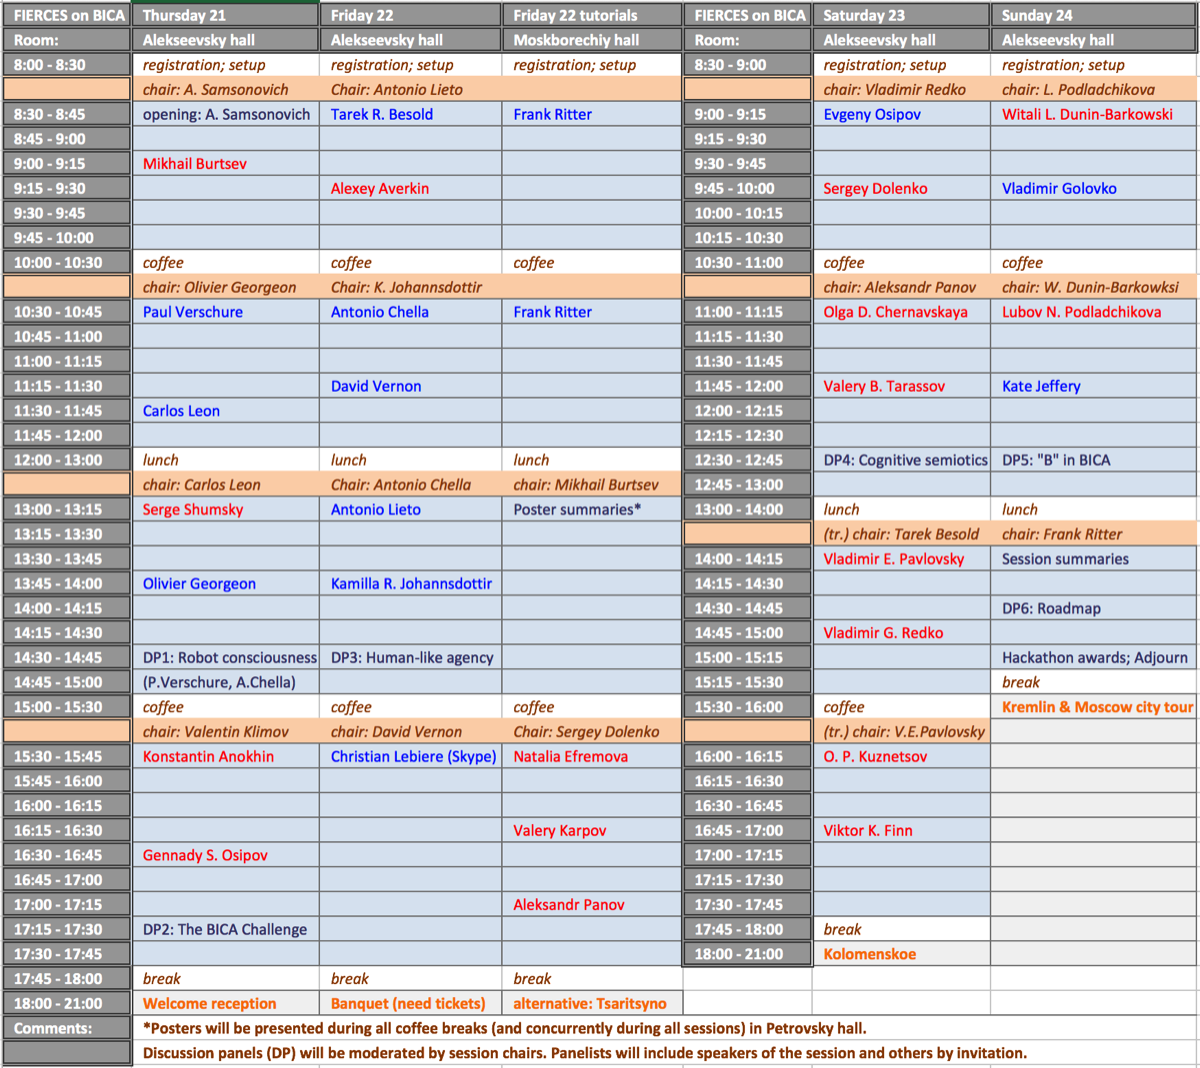
\includegraphics[width=\textwidth]{02_detail_program}
	\vfill
	

\section{Detailed Program}
	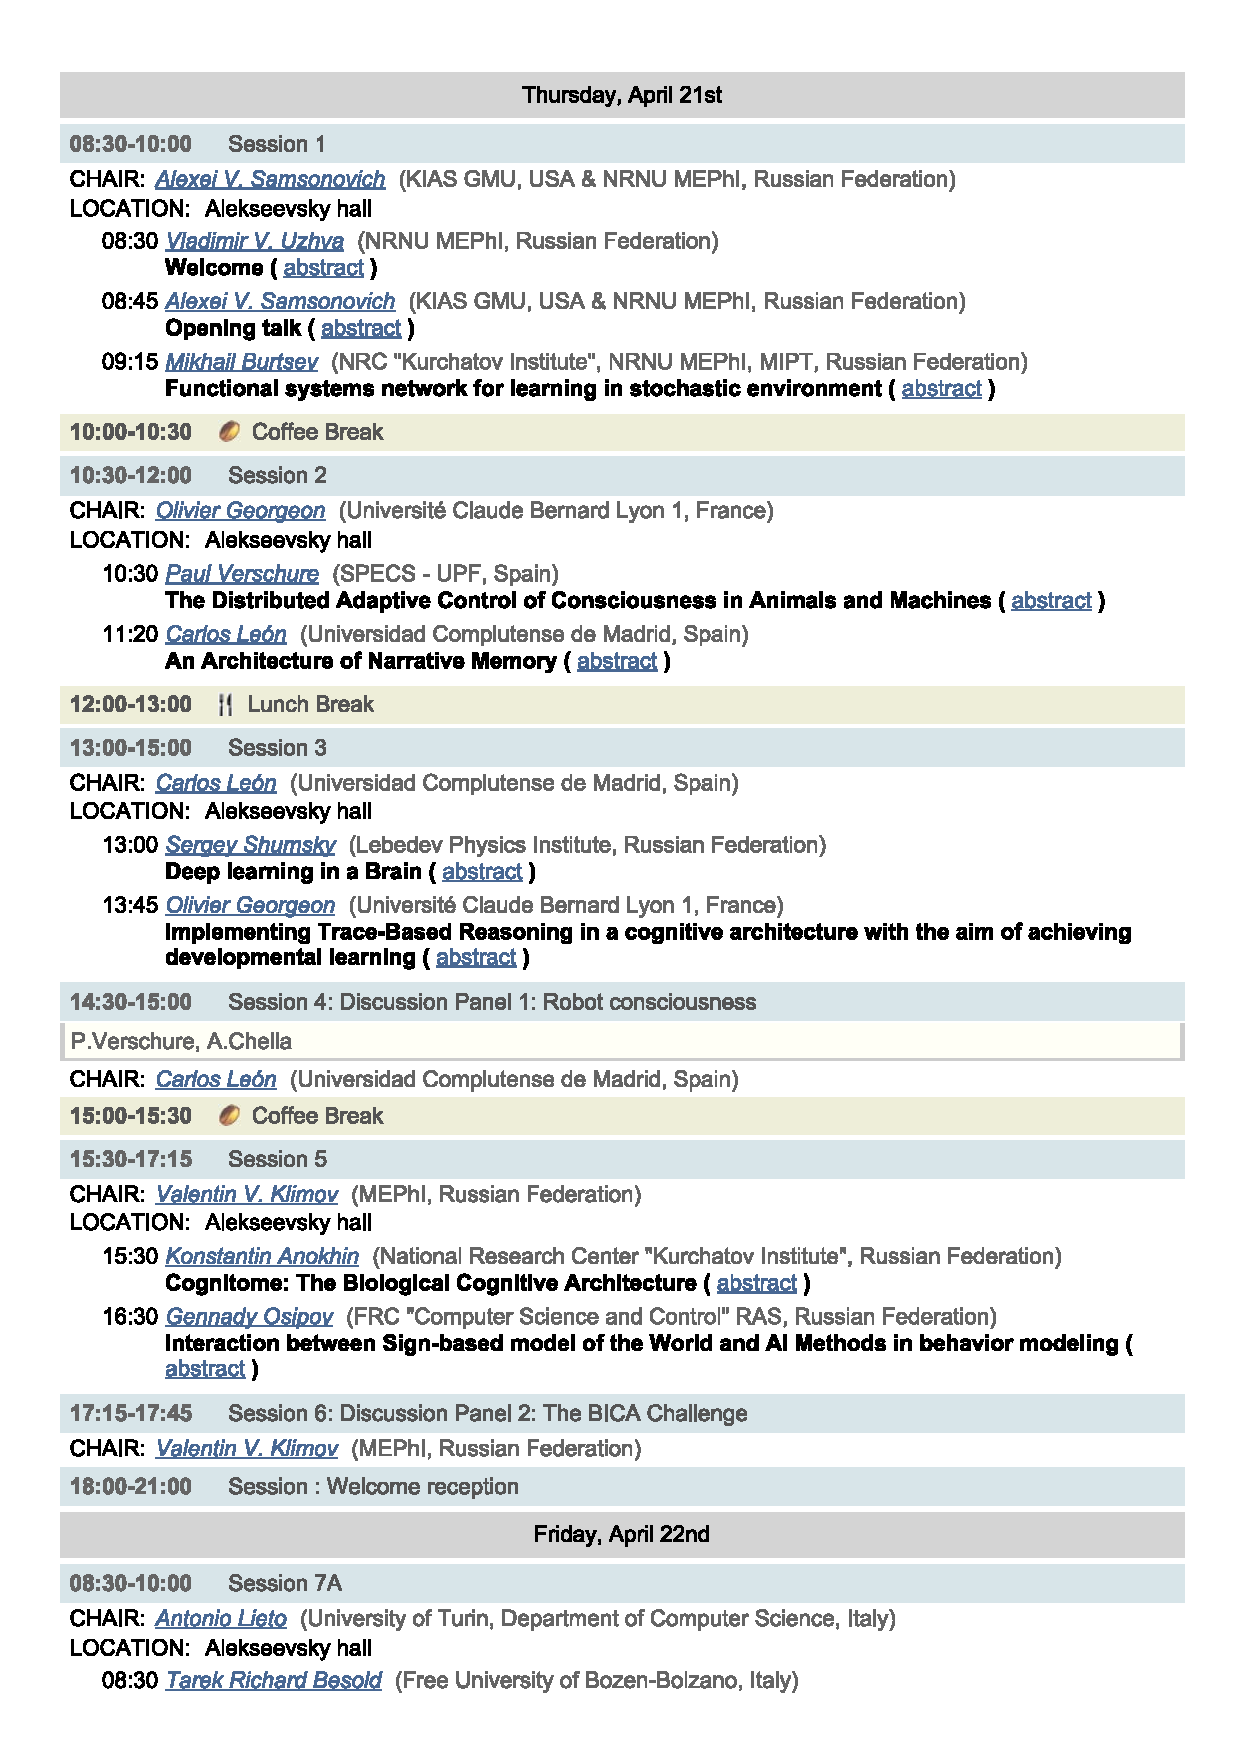
\includegraphics[width=\textwidth, page=1]{02_full_program}
	\includegraphics[width=\textwidth, page=2]{02_full_program}
	\includegraphics[width=\textwidth, page=3]{02_full_program}
	\includegraphics[width=\textwidth, page=4]{02_full_program}


%----------------------------------------------------------------------------------------
%	CHAPTER 3
%----------------------------------------------------------------------------------------

\chapterimage{03_head_venue}

\chapter{Venue}

The School venue is the hotel Intourist-Kolomenskoe, Moscow, Russia. Its beautiful 14-floor building is located near the highway Kashyrskoye – next to MEPhI. The surrounding is quiet and peaceful, with the Moscow River in the heart of the beautiful landscape. Intourist Kolomenskoye offers 259 guest suites, plus a number of meeting rooms and restaurants. All technical sessions will be held in the Alexeevsky hall, the greatest meeting room of the hotel.

\intextfigure{03_hotel_inside}

Intourist Kolomenskoye 4* is a new ultramodern hotel, located near Moscow River, just 10 minutes away from the metro station, which is the part of one of the most important metro line in Moscow. By taking this line, you can reach international airport Domodedovo. Our hotel has 14 levels, every room’s window yield a gorgeous panoramic view on the city and surroundings. The Moscow State Integrated Art and Historical Architectural and Natural Landscape Museum-Reserve Kolomenskoye is former royal estate situated not far from the hotel. There you may see historical architecture monuments year-round. 

\vfill
\intextfigure{03_hotel_13f}

\paragraph{Hotel Services}
\begin{itemize}
	\item \parbox[t]{\dimexpr\textwidth-\leftmargin}{
		\vspace{-2.5mm}				
		\begin{wrapfigure}{c}{0.45\textwidth}
			\vspace{-25pt}				
			\centering				
			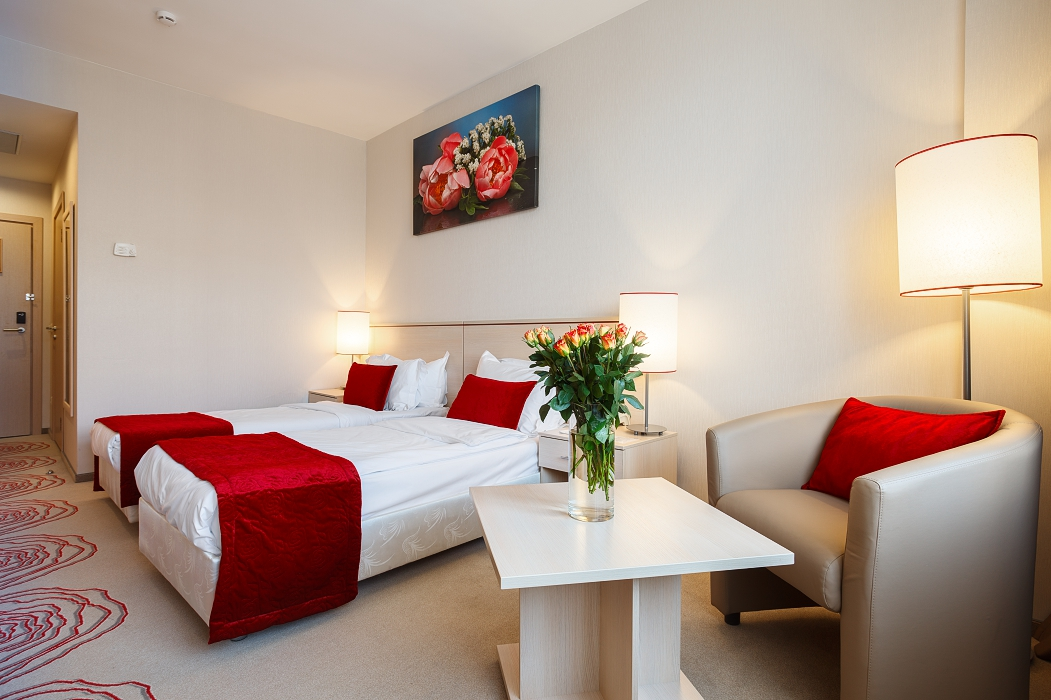
\includegraphics[width=0.3\textwidth]{03_hotel_suite}
		\end{wrapfigure}
		Restaurant and lobby bar
	}
	\item 4 halls for conferences, seminars, banquets
	\item free Wi-Fi throughout the hotel
	\item underground and surface parking
	\item laundry and dry cleaning
	\item transport services
	\item free Shuttle to/from "Kashirskaya" metro station
\end{itemize}

\paragraph{The distance from airports and railway stations}
\begin{itemize}
	\item \parbox[t]{\dimexpr\textwidth-\leftmargin}{
		\vspace{-2.5mm}				
		\begin{wrapfigure}{c}{0.45\textwidth}
			\vspace{-25pt}				
			\centering				
			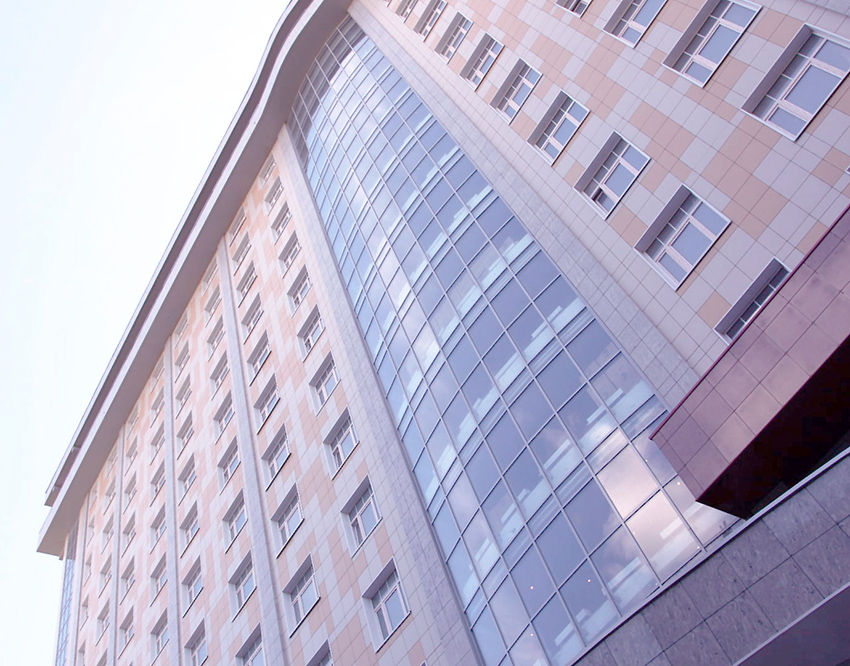
\includegraphics[width=0.3\textwidth]{03_hotel_outside}
		\end{wrapfigure}
		Domodedovo – 30 km (18,6 ml)
	}
	\item Vnukovo – 34 km (21,1 ml)
	\item Sheremetyevo – 45 km (28 ml)
	\item Paveletsky railway station – 9 km (5,6 ml)
	\item Kievsky railway station – 15 km (9,3 ml)
\end{itemize}

\par\bigskip
\par\bigskip
\begin{description}
	\item[Phone] +7-495-662-1001
	\item[Email] bron@intourist-kolomenskoe.ru
	\item[Web] http://intourist-kolomenskoe.ru/en/
	\item[Address] Kashyrskoye shosse, 39b, Moscow, 115478, Russia
\end{description}

%----------------------------------------------------------------------------------------
%	CHAPTER 4
%----------------------------------------------------------------------------------------

\chapterimage{04_head_moving_around}

\chapter{Moving around}

\section{Local area}

\begin{enumerate}
	\item National Research Nuclear University MEPhI
		\begin{description}
			\item[Address] 31 Kashirskoye shosse, Moscow, 115404
			\item[Telephone] +7 (495) 788-56-99
	     	\item[E-mail] rector@mephi.ru
	     	\item[Web-site] https://mephi.ru/eng/
		\end{description}

    \item Intourist Kolomenskoye Hotel
    	\begin{description}
    		\item[Address] 39b Kashirskoye shosse, Moscow, 115409
    		\item[Telephone] +7 (495) 662-10-01
    		\item[E-mail] bron@intourist-kolomenskoe.ru
    		\item[Web-site] http://intourist-kolomenskoe.ru/en/
    	\end{description}
	
	\item MEPhI Dorm
	    \begin{description}
	    	\item[Address] 8k2 Proletarskiy prospect, Moscow
	    	\item[Telephone] +7 (495) 788-56-99
	    \end{description}
	
    \item Kolomenskoe Park
        \begin{description}
        	\item[Address] 39 Andropova Avenue, Moscow
        	\item[Telephone] +7 (495) 232-61-90
        	\item[Web-site] http://mgomz.com/kolomenskoe
        \end{description}

	Permanent Expositions opening hours:
		\begin{itemize}
			\item Expositions are open daily except Monday, from 11.00 to 19.00
			\item Expositions at the Palace of the Tsar Alexey Mikhailovich are open at weekends, from 10.00 to 19.00
		\end{itemize}
		
	\item Shopping \& entertainment center «Moskvorechie»
	\begin{description}
		\item[Address] 26, Kashirskoe highway, Moscow
		\item[Telephone] +7(495) 966-00-02
		\item[E-mail] trk@moskvorechije.ru
		\item[Web-site] http://www.moskvorechije.ru/en/
		\item[Open hours] daily, 10:00 a.m. - 22:00 p.m.
	\end{description}
	
	The three-storeyed center accommodates 110 stores, 15 popular restaurants and cafes, a big supermarket, entertainment center with the cinema and Kids’ Learning Center.	
		
	\item Sberbank
	    \begin{description}
	    	\item[Address] 6k1 Proletarskiy prospect, Moscow
	    	\item[Telephone] +7(499) 324-07-55
	    	\item[Open hours] 08:30 - 19:30
	    \end{description}

    \subsection{Supermarkets}
    
	    \item Grocery supermarket “Klen”
	       	\begin{description}
	       		\item[Address] 31k2, Moskvorechie st., Moscow
	       		\item[Telephone] +7 (499) 320-32-22
	       		\item[Open hours] 24/7
	       	\end{description}
	
		\item Grocery supermarket “Pyaterochka”
	       	\begin{description}
	       		\item[Address] 42k1 Kashirskoe sh., Moscow
	       		\item[Telephone] +7 (800) 555-55-05
	       		\item[Open hours] 9:00 – 23:00
	       		\item[Web-site] http://www.pyaterochka.ru/  
	       	\end{description}
	      
    \subsection{Restaurants, cafes and bars}
    	
    	\item Art-café Goncharov
	    	\begin{description}
	    		\item[Address] 23 Moskvorechie st., Moscow
	    		\item[Web-site] http://mskr.ru/art-kafe-goncharov/
	    	\end{description}
    	
    	\item Restaurant Guel 
		   	\begin{description}
		   		\item[Address] 40, Kashirskoe sh., Moscow
		   		\item[Web-site] http://www.rest-guel.ru/
		   	\end{description}    
    	
    	\item Bar Killfish
	    	\begin{description}
	    		\item[Address] 42/1, Kashirskoe sh., Moscow
	    		\item[Web-site] http://killfish.ru/
	    		\item[Open hours] 15:00 - 02:00
	    	\end{description} 
\end{enumerate}

\subsection{Other places nearby}

\begin{itemize}
	
	\item Restaurant Tanuki 
	\begin{description}
		\item[Address] 46, Kashirskoe sh., Moscow
		\item[Web-site] http://www.tanuki.ru/en/
	\end{description}
	
	\item Supermarket “Azbuka vkusa”
	\begin{description}
		\item[Address] 78, Kashirskoe sh., Moscow
		\item[Open hours] 24/7
		\item[Web-site] http://www.av.ru/  
	\end{description}
	
\end{itemize}

\begin{figure}[H]
	\begin{center}
		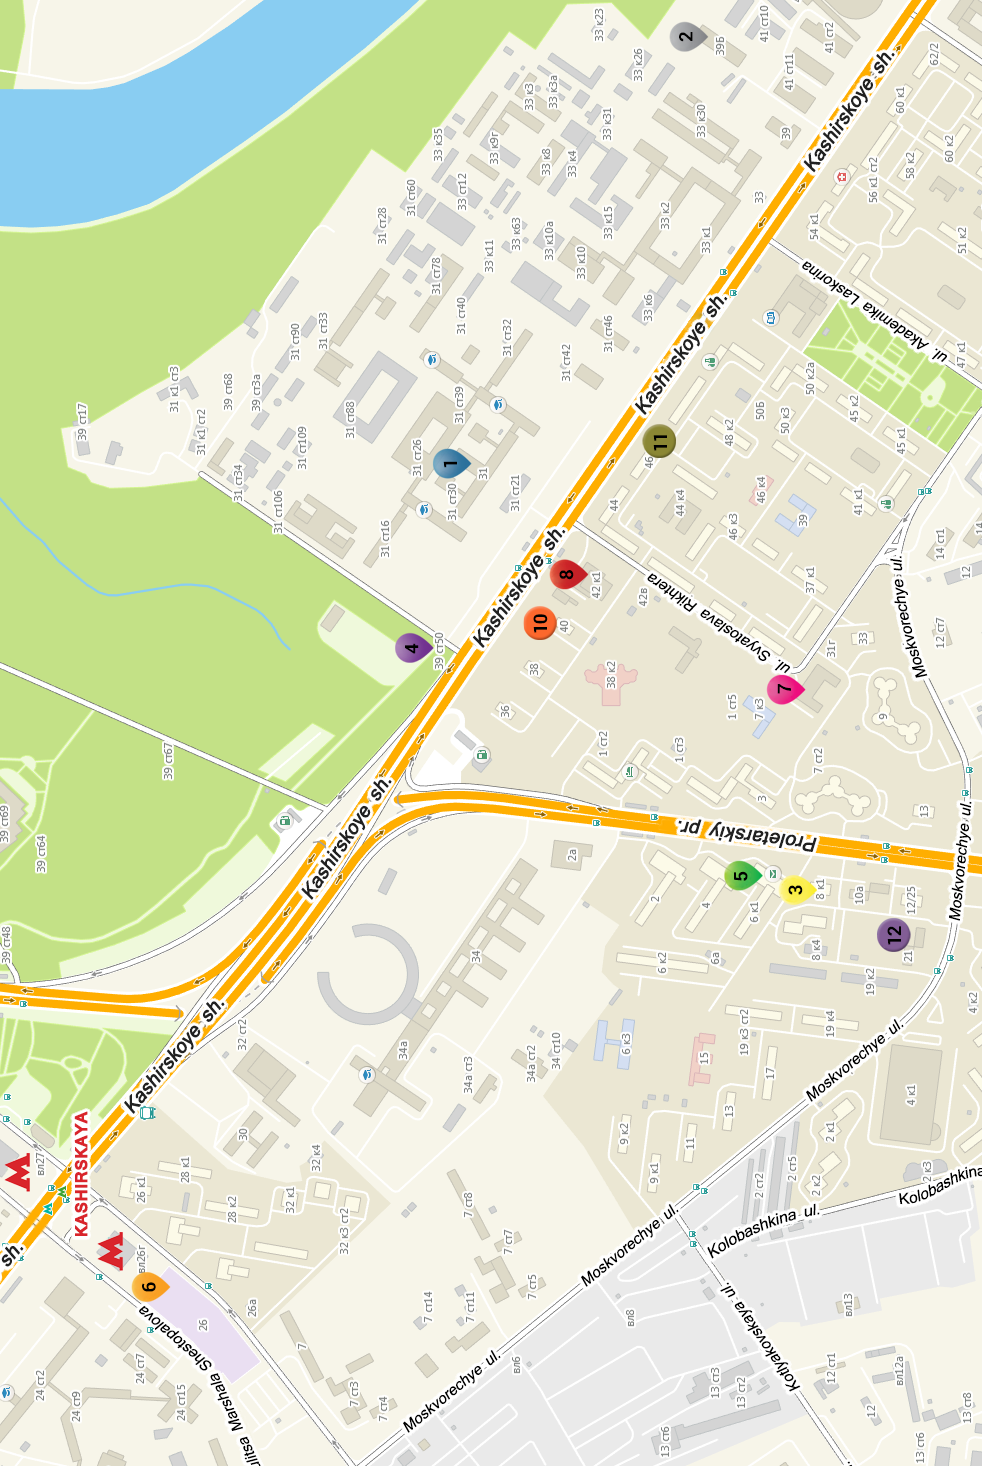
\includegraphics[width=\paperwidth - 2cm]{04_local_map}
	\end{center}
\end{figure}

\section{Recommended museums, art galleries, and parks}

\begin{enumerate}
	\item The State Historical Museum
		\begin{description}
			\item[Web-site] www.shm.ru/en/
			\item[Address] 1, Red Square, Moscow, 103012, Russia 
			\item[Transport] Metro Stations Okhotny Ryad, Ploshad Revolutsii, Teatralnaya Ploshad
			\item[Opening hours] Daily from 11.00 to 19.00, closed on Tuesdays
		\end{description}

	\item 	Yuri Orlov Palaeontological Museum
		\begin{description}
			\item[Web-site] http://www.paleo.ru/museum/ 
			\item[Address] 123, Profsoyuznaya Ulitsa, Moscow, 117647, Russia 
			\item[Transport] From Teply Stan Metro station it's one stop on any form of transport, or 5-7 minutes on foot.
			\item[Opening hours] Wednesday to Friday - 10:00 to 16:00, Saturday and Sunday - 10:00 to 18:45, closed Monday and Tuesday
		\end{description}

	\item Moscow State University Zoological Museum
		\begin{description}
			\item[Web-site] http://zmmu.msu.ru/en
			\item[Address] 6, Bol'shaya Nikitskaya ulitsa, Moscow, 103009, Russia 
			\item[Transport] Okhotny Ryad or Aleksandrovsky Sad Metro stations
			\item[Opening hours] Tuesday to Sunday - 10:00 to 17:00. Monday - closed. The museum is closed on the last Tuesday of each month
		\end{description}

	\item Cosmonautics Memorial Museum
		\begin{description}
			\item[Web-site] http://www.kosmo-museum.ru/
			\item[Address] 111, Prospekt Mira, Moscow, 129515, Russia 
			\item[Transport] VDNKh Metro station
			\item[Opening hours] Daily - 10:00 to 18:00, except Mondays and the last Friday of each month
		\end{description}
	
	\item Andrei Rublev Museum of Ancient Russian Art
			\begin{description}
				\item[Web-site] http://www.rublev-museum.ru/ 
				\item[Address] 10, Andronevskaya Ploshad, Moscow, 105120, Russia 
				\item[Transport] Ploshad' Il'icha and Taganskaya Metro stations
				\item[Opening hours] 11:00 to 18:00, except Wednesdays and the last Friday of each month
			\end{description}
			
	\item State Tretyakov Gallery
	\begin{description}
		\item[Web-site] http://www.tretyakovgallery.com
		\begin{itemize}
			\item Main Gallery
				\begin{description}
					\item[Address] 10, Lavrunshkensky Pereulok, Moscow, 119017, Russia 
					\item[Transport] Tretyakovskaya or Novokuznetskaya Metro stations
			    \end{description}
   			\item House of Artists
	   			\begin{description}
					\item[Address] 10/4, Ulitsa Krymsky Val, Moscow, 119049, Russia 
					\item[Transport] From Park Kulturi or Oktyabr'skaya Metro station take trolleybuses 10 or B to the Central Park of Culture and Leisure stop
	   			\end{description}
		\end{itemize}
		\item[Opening hours] Daily from 10:00 – 19:00 (20:00), except Mondays 
	\end{description}
	
	\item State Pushkin Museum of Visual Art
		\begin{description}
			\item[Web-site] http://www.arts-museum.ru/
			\item[Address] 12, Ulitsa Volkhonka, Moscow, 121019, Russia 
			\item[Transport] Kropotkinskaya Metro station
			\item[Opening hours] Tuesday to Sunday - 10:00 to 18:00, closed on Mondays.
		\end{description}

	\item The Palace of the Romanov Boyars
		\begin{description}
			\item[Web-site] http://www.museum.ru/M415 
			\item[Address] 10, Ulitsa Varvarka, Moscow, 103012, Russia 
			\item[Transport] Kitai Gorod Metro Station
			\item[Opening hours] Daily from 10:00 to 17:00, closed on Tuesdays and the first Monday of each month
		\end{description}

	\item Izmailovsky Park
	\begin{description}
		\item[Web-site] http://www.izmailovsky-park.ru/ 
		\item[Getting there] The main entrance to the park, the market and Silver Island are located next to Izmailovsky Park Metro Station and the Izmailovo Hotel Complex. However, you can also go to Izamailovskaya Metro Station - actually located above-ground - and enter along one of the park's most picturesque alleys.
	\end{description}
	
	\item Kolomenskoe park
		\begin{description}
			\item[Web-site] http://mgomz.com/
			\item[Getting there] The main entrance to the park is about 10 minutes' walk from Kolomenskaya Metro Station
			\item[Opening hours] Daily from 09:00 to 19:00 (from April till August to 22:00)
		\end{description}
	
	\item Gorky Park
		\begin{description}
			\item[Web-site] http://www.park-gorkogo.com/ 
			\item[Address] 9, Krymskiy Val, Moscow, 117049, Russia.
			\item[Getting there] Park Kultury or Oktiabrskaya Metro Stations.
			\item[Opening hours] Daily from 10:00 to 22:00 (most of the rides are closed in the winter)
		\end{description}

	\item The All-Russian Exhibition Center (VVTs)
		\begin{description}
			\item[Web-site] https://vdnh.ru/ 
			\item[Getting there] VDNKh Metro Station
		\end{description}

	\item Victory Park on Poklonnaya Gora
		\begin{description}
			\item[Web-site] http://www.poklonnaya-gora.ru/ 
			\item[Getting there] Park Pobedy Metro Station
		\end{description}
		
\end{enumerate}

\section{Where to eat and to have a drink?}

\subsection{Famous addresses for gastronomic food or panoramic view, or both}

\begin{enumerate}
	
	\item Café Pushkin 
		\begin{description}
			\item[Address] 26A Tverskoy Boulevard, Moscow
			\item[Web-site] http://www.cafe-pushkin.ru/
		\end{description}
	
	\item Gallery Café
		\begin{description}
			\item[Address] 27 Ulitsa Petrovka, Moscow 127031
			\item[Web-site] http://cafe-gallery.ru
		\end{description}
	
	\item Restaurant Sixty
		\begin{description}
			\item[Address] Moscow International Business Center, Federation Tower, 60th floor, Presnenskaya emb., 12
			\item[Web-site] http://en.ginza.ru/msk
		\end{description}

	\item Restaurant Seventh Heaven 
		\begin{description}
			\item[Address] 15 Ak. Korolyova St., Moscow 
			\item[Web-site] http://www.tvtower.ru/51\_Restoran/eng/ 
		\end{description}

	\item Restaurant O2 Lounge
		\begin{description}
			\item[Address] 3 Tverskaya St., Moscow 
			\item[Web-site] http://www.ritzcarlton.com/en/hotels/europe/moscow/hotel-overview/
		\end{description}
	
\end{enumerate}

\subsection{Streets/Areas with Typical Restaurants}

\begin{enumerate}
	
	\item Arbat Street - Cafes and places to wine and dine are everywhere -different kitchens (Russian, Italian, Caucasian, Japanese, American)
		\begin{description}
			\item[Address] Smolenskaya and Arbatskaya (Dark blue line) metro stations, 10 min walk from the Kremlin. The street stretches for about 1 km between these two stations
		\end{description}
	\item Kamergersky Pereulok - A historical street where the composer Sergei Prokofiev and a poet Nikolai Aseyev lived
		\begin{description}
			\item[Address] Teatralnaya (Dark green line) and Ohotniy ryad (Red line) metro stations, the street runs perpendicular to the Moscow Operetta Theatre
		\end{description}
	\item Tverskaya Ulitsa - The city's central thoroughfare since the Middle Ages, home to prestigious shops and restaurants, and has long been the centre of Moscow's theatreland. 
		\begin{description}
			\item[Address] Tverskaya metro station (Dark green line). The street runs Northwest from the central Manege Square
		\end{description}
		
\end{enumerate}
\newpage
\section{Most popular and suggested places to visit (with a brief description)}
	
	\textbf{Red Square} remains, as it has been for centuries, the heart and soul of Russia. Few places in the world bear the weight of history to the extent that Moscow's central square does. From the 16thCentury \textbf{St. Basil's Cathedral} - one of the most famous pieces of architecture in the world - to the constructivist pyramid of\textbf{ Lenin's Mausoleum}, Red Square is rich in symbols of Russia's turbulent and intriguing past.
	
	\intextfigure{04_RedSquare}
	
	Nearby is the \textbf{Gum store}, \textbf{State Historical Museum} and \textbf{The Kremlin} which is the former royal citadel and currently the official residence of the President of Russia.
		\begin{description}
			\item[Address] Red Square (Krasnaya ploshchad), Moscow 109012
			\item[Transport] Okhotny Ryad or Ploshad  metro stations
		\end{description}
		
	\intextfigure{04_ChristTheSaviour}
	
	One of the most imposing and controversial buildings in Russia, the resurrected \textbf{Cathedral of Christ the Saviour} has had a short but turbulent history. It was originally commissioned after the defeat of Napoleon, but work did not begin on its construction until 1839. Designed by the great St. Petersburg architect Konstantin Ton, who was also responsible for the Grand Kremlin Palace and the Kremlin Armoury and whose church designs pioneered the Byzantine-revival style, the cathedral was erected, for maximum effect, on the embankment only a few minutes' walk from the Kremlin. Sadly, this entailed the destruction of the medieval Alekseevskiy Convent, a course of events which lends an intriguing irony to the cathedral's own fate.
	
	\intextfigure{04_Kolomenskoe}
	
	\textbf{Kolomenskoe park} is one of the most beautiful places in all of Moscow. Although only a short metro ride from the center, and situated close to one of the city's most industrialized areas, the park and its awe-inspiring buildings are so steeped in history that not even the Kremlin itself can quite so well evoke the Russia of old.
	
	\intextfigure{04_Kolomenskoe2}
	
	Arriving at Kolomenskoe along a street of drab Soviet tower blocks, you are first confronted by a rather gaudy collection of "medieval" sideshows and souvenir booths, and part of the magic of the experience is the way that this display of touristy tackiness fades from your memory the further you get into the tranquil, rugged beauty of the park proper.
	
	\intextfigure{04_Garage}
	
	\textbf{Garage Museum of Contemporary Art} is an independent platform for new thinking.Through an extensive program of exhibitions, research, education, and publishing, Garage reflects on current developments in Russian and international culture, creating opportunities for public dialogue and the production of new work and ideas.
	It’s situated in the \textbf{Gorky Park}, a central park in Moscow, named after Maxim Gorky, a Russian and Soviet writer, a founder of the socialist realism literary method. 
	The the German rock band Scorpions were inspired to write the song on a visit to Moscow in 1989, and the opening lines refer to the city's landmarks:
	\begin{quotation}
		\begin{center}
		\textit{I follow the Moskva\\
				Down to Gorky Park\\
				Listening to the wind of change}
		\end{center}
	\end{quotation}
	
	\intextfigure{04_Arbat}
	
	\textbf{Arbat Street} is a pedestrian street about one kilometer long in the historical centre of Moscow. The Arbat has existed since at least the 15th century, thus laying claim to being one of the oldest surviving streets of the Russian capital. Originally the street formed part of an important trade route and was home to a large number of craftsmen.
	
	\intextfigure{04_Tverskaya}
	
	The city's central thoroughfare since the Middle Ages, \textbf{Tverskaya Street}  is now home to prestigious shops and restaurants, and has long been the centre of Moscow's theatreland. Nowadays Tverskaya is one of the Moscow's main streets, which runs uphill from opposite the north end of Red Square.
	
	\intextfigure{04_Theatre}
	
	\textbf{The Bolshoi Theatre} is a historic theatre in Moscow, Russia, designed by architect Joseph Bové, which holds performances of ballet and opera. 
	The Bolshoi Ballet and Bolshoi Opera are amongst the oldest and most renowned ballet and opera companies in the world. It is by far the world's biggest ballet company, having more than 200 dancers. The theatre is the parent company of The Bolshoi Ballet Academy, a world-famous leading school of ballet. It has a branch at the Bolshoi Theatre School in Joinville, Brazil. 
	The main building of the theatre, rebuilt and renovated several times during its history, is a landmark of Moscow and Russia.
	
	\intextfigure{04_VVTs}
	
	\textbf{The All-Russian Exhibition Center (VVTs)} is a bizarre juxtaposition: part agricultural fair, part trade expo, part shopping centre and part street market, with amusements as diverse as paint-balling and camel rides - as well as the ubiquitous slot-machine arcades - on offer in various parts of the grounds. The park itself is an intriguing example of 20th century landscaping and, even if they are a little the worse for wear, the buildings are still preposterously magnificent. The VVTs is truly unique, and well worth a visit, especially as there is plenty more to be seen nearby, including the wonderful \textbf{Cosmonautics Musuem}, \textbf{the Ostankino TV Tower}, and the very different delights of the Ostankino Park.
	
	\intextfigure{04_Tsaritsyno}
	
	\textbf{Tsaritsyno park} is the only 18th-century architectural ensemble of such dimensions in Russia. Around the grand palace, in the park there are a number of pavilions, pergolas, arbours, artificial grottos, decorative bridges, and a Russian Orthodox temple “Source of Life”, as well as a modern recreation center with an upscale restaurant. For a long time most buildings were ruined (and used for rock climbing). In 2005-2007 most buildings were extensively restored and completed: roofs, interiors and decorations have been added and their historical appearance has been altered. The atrium of the “Bread House” is used for concerts of Moscow musicians. 
	The park grounds contain the group of burial mounds (Kurgans) that belong to the Early Slavs tribe Vyatichs dated to the 11th-13th century
	
\section{Airports}

\subsection{Domodedovo Airport}
\paragraph{Public transport}
\subparagraph{Aeroexpress}
\begin{itemize}
	\item Route time ~50 min
	\item From Paveletsky Railway Station
	\item 6.00-0.30 (every 30 min)
	\item 470 rub
\end{itemize}

\subparagraph{Train}
\begin{itemize}
	\item Route time ~70 min
	\item From Paveletsky Railway Station
	\item 4.45 - 23.00
	\item 130 rub
\end{itemize}

\subparagraph{Bus 308}
\begin{itemize}
	\item Route time ~35 min
	\item From Domodedovskaya subway station
	\item 6.00-0.00 (every 15 min)
	\item 80 rub + luggage
\end{itemize}

\subparagraph{Route taxi 308}
\begin{itemize}
	\item Route time ~35 min
	\item From Domodedovskaya subway station
	\item 6.00-0.00 (every 15 min)
	\item 0.00-6.00 (every 40 min)
	\item 120 rub
\end{itemize}

\paragraph{By car}
\subparagraph{A105 highway}
\begin{itemize}
	\item From Kashirskoye Highway 
\end{itemize}

\subsection{Sheremetyevo Airport}
\paragraph{Public transport}

\subparagraph{Aeroexpress}
\begin{itemize}
	\item Route time ~50 min
	\item From Paveletsky Railway Station
	\item 5.30-0.30 (every 30 min)
	\item 470 rub
\end{itemize}

\subparagraph{Route taxi 949}
\begin{itemize}
	\item Route time ~50 min
	\item From Rechnoy Vokzal subway station
	\item 6.45-21.45
	\item 75 rub
\end{itemize}

\subparagraph{Bus 851}
\begin{itemize}
	\item Route time ~50 min
	\item From Rechnoy Vokzal subway station
	\item 5.40-0.45
	\item 50 rub
\end{itemize}

\subparagraph{Route taxi 948}
\begin{itemize}
	\item Route time ~50 min
	\item From Planernaya subway station
	\item 6.45-21.45
	\item 75 rub
\end{itemize}

\paragraph{By car}
\subparagraph{Sheremetyevskoye Highway}
\begin{itemize}
	\item From Leningradskoye Highway
\end{itemize}

\subsection{Vnukovo Airport}
\paragraph{Public transport}

\subparagraph{Aeroexpress}
\begin{itemize}
	\item Route time ~40 min
	\item From Kievsky Railway Station
	\item 6.00-0.00 (every hour)
	\item 470 rub
\end{itemize}

\subparagraph{Bus 611c}
\begin{itemize}
	\item Route time ~40 min
	\item From Troparyovo and Yugo-Zapadnaya subway stations
	\item 5.00-1.00
	\item 50 rub
\end{itemize}

\subparagraph{Bus 611}
\begin{itemize}
	\item Route time ~40 min
	\item From Troparyovo and Yugo-Zapadnaya subway stations
	\item 7.00-23.00
	\item 50 rub
\end{itemize}

\subparagraph{Route taxi 45M}
\begin{itemize}
	\item Route time ~50 min
	\item From Yugo-Zapadnaya subway station
	\item 7.00-22.30
	\item 100 rub
\end{itemize}

\paragraph{By car}
\subparagraph{M3 highway}
\begin{itemize}
	\item From Kievskoe Highway
\end{itemize}

\section{Moscow Metro Map}
\vspace{20pt}
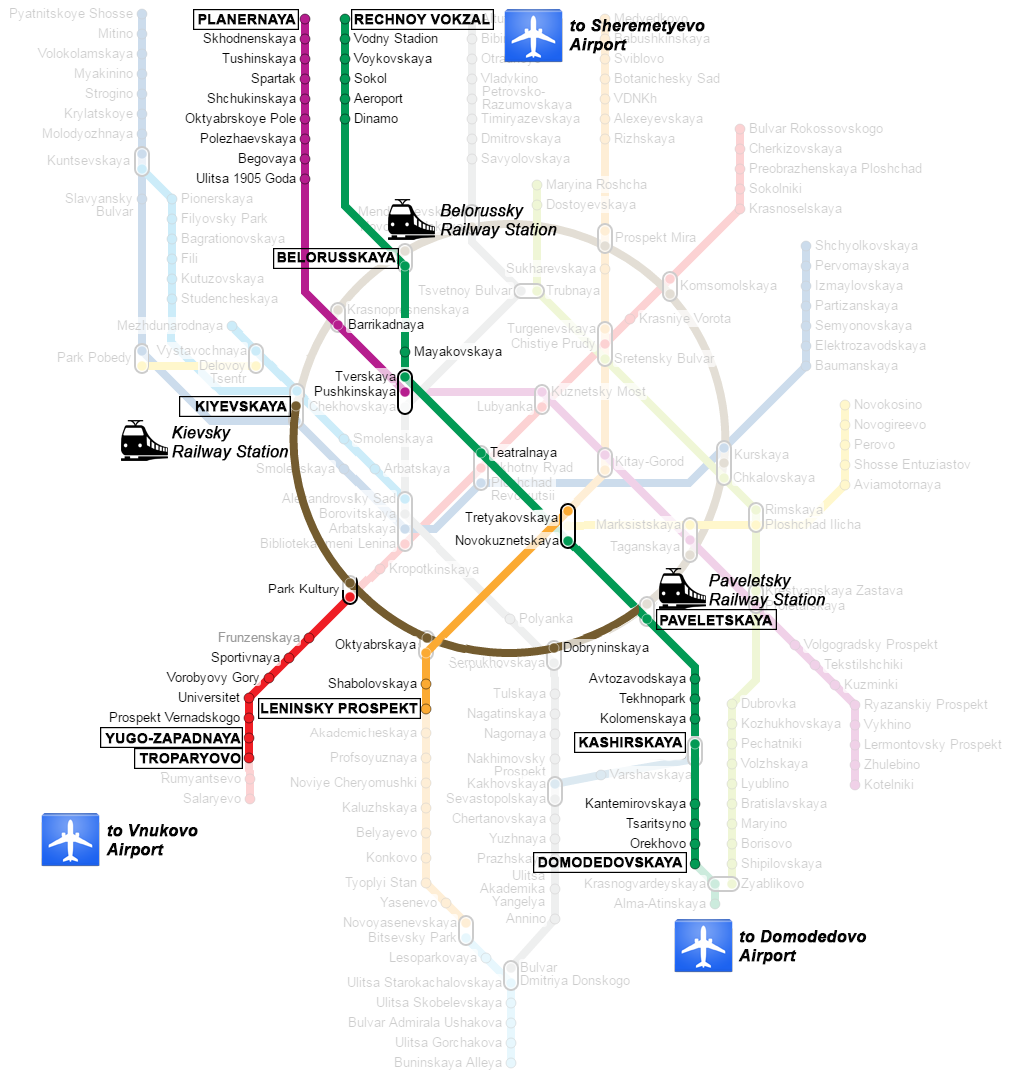
\includegraphics[width=\textwidth]{04_metro_map}

%\intextfigure{04_metro_map}

%----------------------------------------------------------------------------------------
%	CHAPTER 5
%----------------------------------------------------------------------------------------

\chapterimage{05_head_sponsors}

\chapter{Sponsors and Committees}

\section{Sponsor}
\paragraph{Russian Science Foundation}
Russian Science Foundation was established on the initiative of the President of the Russian Federation to support basic research and development of leading research teams in different fields of science. Legal status, powers, functions, proprietary rights and governance of the Foundation are determined by the Federal Law "On the Russian Science Foundation and Amendments to Certain Legislative Acts of the Russian Federation."

\begin{wrapfigure}{r}{0.5\textwidth}
	\begin{center}
		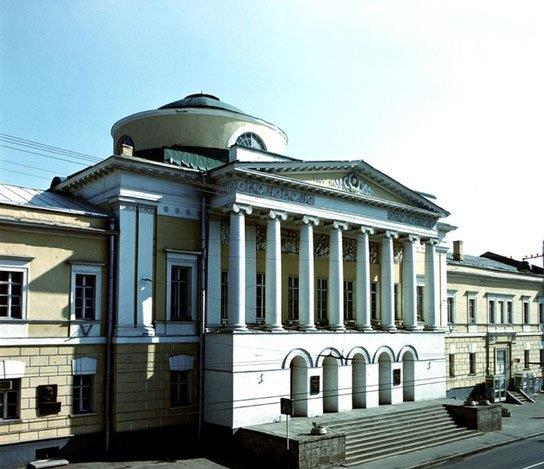
\includegraphics[width=\paperwidth - 8.5cm]{05_rsf-building}
	\end{center}
\end{wrapfigure}

To achieve its goals, the Foundation selects science and technology programs and projects that fall under certain propriety categories, and does so on a competitive basis. Among these priorities are basic research initiatives by research groups or individual scientists, or members of the higher education teaching staff; development of scientific organizations and institutions of higher education, creation of world-class departments and laboratories in scientific organizations and educational institutions, development of experimental facilities for scientific research.

The governance structure of the Foundation is set up by the Federal Law: Supervisory Board, Management board and Director General. The Federal Law sets out a  procedure for formation of these bodies as well as defines their authority. In order to provide the Foundation with the necessary expertise, the Federal law provides for creation of Review Panels acting as advisory bodies of the Foundation. Control over financial and economic activities of the Foundation is exercised by the Audit Committee of the Foundation. In accordance with the Federal Law, Russian Science Foundation submits the annual report for consideration of the President of the Russian Federation and the Government of the Russian Federation.

\vfill

\paragraph{Co-organizers}
	\begin{itemize}
		\item National Research Nuclear University MEPhI
		\item BICA Society
	\end{itemize}

\section{Core Organizing Committee}

\subsection{General Chair}
	Valentin V. Klimov (MEPhI, Moscow)

\subsection{Co-Chairs}
	\begin{itemize}
		\item Andrey M. Zagrebayev (MEPhI, Moscow)
		\item Olga A. Mishulina (MEPhI, Moscow)
		\item Vladimir G. Redko (SRI for System Analysis RAS, Moscow)
	\end{itemize}

\subsection{International Committee Members}
	\begin{itemize}
		\item Antonio Chella (University of Palermo, Italy)
		\item Olivier Georgeon (LIRIS, University of Lyon, France)
		\item Kamilla R. Johannsdottir (University of Reykjavík, Iceland)
		\item Christian Lebiere (Carnegie Mellon University, USA)
		\item Frank Ritter (Penn State University, USA)
		\item Junichi Takeno (Meiji University, Japan)
		\item Jan Treur (VU University Amsterdam, The Netherlands)
	\end{itemize}

\subsection{Local Committee Chair}
	Aleksandr I. Panov (FRC “Computer Science and Control” RAS, Moscow)
	
\subsection{Local Committee Members}
	\begin{multicols}{2}
		\begin{itemize}
			\item Galina A. Beshlebnova (SRI for System Analysis RAS, Moscow)
			\item Artyom A. Chernyshov (MEPhI, Moscow)
			\item Ilya Sukonkin (MEPhI, Moscow)
			\item Anita Balandina (MEPhI, Moscow)
			\item Anastasiya Kostkina (MEPhI, Moscow)
		\end{itemize}
	\end{multicols}
	
\paragraph{Congress-centre MEPhI}
		\begin{itemize}
			\item 
			\parbox[t]{\dimexpr\textwidth-\leftmargin}{
				\vspace{-2.5mm}				
				\begin{wrapfigure}{c}{0.6\textwidth}
					\vspace{-2.5mm}
					\centering				
					
\includegraphics[width=0.3\textwidth]{05_Logo_Congress}
				\end{wrapfigure}
				Polina Tolstaya
			}
			\item Vera Inkina
			\item Aldar Dzhambinov
			\item Artem Tyutyunnikov
			\item Anton Gerasimchuk
			\item Nikita Matveev
			\item Tamerlan Alborov
		\end{itemize}
	
\subsection{Program Committee Chairs}
	\begin{itemize}
		\item Alexei V. Samsonovich (George Mason University, USA; MEPhI, Moscow)
		\item Valentin V. Klimov (MEPhI, Moscow)
		\item Galina Rybina (MEPhI, Moscow)
	\end{itemize}


\subsection{Program Committee Members}
	\begin{multicols}{2}
		\begin{itemize}
			\item Karolin Abdul-Aziz
			\item Myriam Abramson
			\item Tsvi Achler
			\item Samuel Adams
			\item Giovanni Adorni
			\item Reza Ghasem Aghaiee
			\item Colin Allen
			\item Leonardo Almada
			\item Yiannis Aloimonos
			\item Heather Ames
			\item Michael Anderson
			\item Konstantin Anokhin
			\item Panos Antsaklis
			\item Kenji Araki
			\item Itamar Arel
			\item Raul Arrabales
			\item Roger Azevedo
			\item Joscha Bach
			\item Tatiana Baidyk
			\item Balaji Balasubramaniam
			\item Allan Barros
			\item Paul Baxter
			\item Gary Berg-Cross
			\item Robert Berwick
			\item Tarek R. Besold
			\item Perrin Bignoli
			\item Gautam Biswas
			\item Zbigniew Bogdanowicz
			\item Peter Boltuc
			\item Jonathan Bona
			\item Gregoire Borst
			\item Tibor Bosse
			\item Michael Brady
			\item Bert Bredeweg
			\item Andrew Browning
			\item Stéphane Bura
			\item Erik Cambria
			\item Andrea Carbone
			\item Aiello Carlucci
			\item Nicholas Cassimatis
			\item Ritu Chadha
			\item Antonio Chella
			\item Wei Chen
			\item Olga Chernavskaya
			\item Yushing Cheung
			\item Robert Clowes
			\item Vasile Coman
			\item Robert Coop
			\item Roberto Cordeschi
			\item Massimo Cossentino
			\item Andrew Coward
			\item Jose Cruz-Albrecht
			\item Artur D'Avila Garcez
			\item Sidney D'Mello
			\item Mike Daily
			\item Christopher Dancy
			\item Son Dao
			\item James Davidson
			\item Hugo De Garis
			\item Haris Dindo
			\item Petre Dini
			\item Simona Doboli
			\item Sergey A. Dolenko
			\item James Eilbert
			\item Chris Eliasmith
			\item Thomas Eskridge
			\item Usef Faghihi
			\item Elena Fedorovskaya
			\item Michele Ferrante
			\item Stanley Franklin
			\item Herve Frezza-Buet
			\item Marcello Frixione
			\item Alexander Frolov
			\item Karl Fua
			\item Salvatore Gaglio
			\item David Gamez
			\item Ross Gayler
			\item Olivier Georgeon
			\item John Gero
			\item Laurie Gibson
			\item Gerd Gigerenzer
			\item Ben Goertzel
			\item Jaime Gomez
			\item Petro Gopych
			\item Sergey Grigoryev
			\item Diane Gromala
			\item Horst-Michael Gross
			\item Helmar Gust
			\item Paul Hasler
			\item Seth Herd
			\item Laura Hiatt
			\item Owen Holland
			\item Ian Horswill
			\item Seyyed Abed Hosseini
			\item Michael Howard
			\item Eva Hudlicka
			\item Dusan Husek
			\item Christian Huyck
			\item Ignazio Infantino
			\item John Irvine
			\item David Israel
			\item Alex P. James
			\item Magnus Johnsson
			\item Benjamin Johnston
			\item Darsana Josyula
			\item Kamilla Jóhannsdóttir
			\item Daniel Kahneman
			\item Nikola Kasabov
			\item Omid Kavehei
			\item Troy Kelley
			\item William Kennedy
			\item Deepak Khosla
			\item Muneo Kitajima
			\item Anastasia Kitsantas
			\item Fabian Koeth
			\item Paul Kogut
			\item Stephen Kosslyn
			\item Jeffrey Krichmar
			\item Jim Kroger
			\item Ulf Krumnack
			\item Oleg Kryshtal
			\item Kai-Uwe Kuehnberger
			\item Dinesh Kumar
			\item Unmesh Kurup
			\item Kenneth Kwok
			\item Giuseppe La Tona
			\item Luis Lamb
			\item Othalia Larue
			\item Richard Lau
			\item Christian Lebiere
			\item David Leibovitz
			\item Jürgen Leitner
			\item Emmanuel Lesser
			\item Alexander Letichevsky
			\item Simon Levy
			\item Antonio Lieto
			\item Mei Yii Lim
			\item Igor Linkov
			\item Giuseppe Lo Re
			\item Shoshana Loeb
			\item Andras Lorincz
			\item Anton Loss
			\item Brad Love
			\item Thomas Lu
			\item Wei Lu
			\item Rose Luckin
			\item Sean Luke
			\item Gaia Lupo
			\item Akshay Maan
			\item Evie Malaia
			\item Maria Malfaz
			\item Riccardo Manzotti
			\item Nadimeh Mazlomian
			\item Thomas McGinnity
			\item Patrick Mcknight
			\item Emanuele Menegatti
			\item Elena Messina
			\item Mitar Milacic
			\item Zaruhi Mnatsakanyan
			\item Derek Monner
			\item Marco Morana
			\item Steve Morphet
			\item Shane Mueller
			\item Catherine Myers
			\item Waseem Naqvi
			\item Daniele Nardi
			\item Sergei Nirenburg
			\item David Noelle
			\item Tatsuya Nomura
			\item Andrew Nuxoll
			\item Henrik Olsson
			\item Andrea Omicini
			\item Marco Ortolani
			\item Jaehyon Paik
			\item Joel Pearson
			\item Charles Peck
			\item David Peebles
			\item Carlo Penco
			\item Jacques Penders
			\item Alfredo Pereira Jr.
			\item Peter Petre
			\item Alex Petrov
			\item Giovanni Pezzulo
			\item Giovanni Pilato
			\item Robinson Pino
			\item Fiora Pirri
			\item R. Pirrone
			\item Zygmunt Pizlo
			\item Vladimir Podladchikov
			\item Roberto Poli
			\item Chris Poulin
			\item Michal Ptaszynski
			\item Paavo Pylkkanen
			\item Dmitri Rachkovskij
			\item Uma Ramamurthy
			\item Anjan Ray
			\item Thomas Recchia
			\item Vladimir Redko
			\item James Reggia
			\item Scott Reilly
			\item Mark Reimers
			\item Frank Ritter
			\item Frederique Robert-Inacio
			\item Paul Robertson
			\item Brandon Rohrer
			\item Edmund Rolls
			\item Pablo Roman
			\item Derek Rose
			\item Paul Rosenbloom
			\item David Rosenbluth
			\item Pier-Giuseppe Rossi
			\item Christopher Rouff
			\item Rafal Rzepka
			\item Swathikiran S
			\item Joseph Salvo
			\item Alexei V. Samsonovich
			\item Fredrik Sandin
			\item Giulio Sandini
			\item Amy Santamaria
			\item Ricardo Sanz
			\item Mohamad Sawan
			\item Michael Schader
			\item Theresa Schilhab
			\item Juergen Schmidhuber
			\item Walt Schneider
			\item Michael Schoelles
			\item Catherine Schuman
			\item Valeria Seidita
			\item Mike Sellers
			\item Ignacio Serrano
			\item Antonio Sgorbissa
			\item Hamed Shahbazi
			\item Sheena Sharma
			\item Alexei Sharpanskykh
			\item Hava Siegelmann
			\item Tomas Singliar
			\item Robert Skopec
			\item Timothy Smith
			\item Javier Snaider
			\item Donald Sofge
			\item Meehae Song
			\item Rosario Sorbello
			\item John Sowa
			\item Narayan Srinivasa
			\item Robert St Amant
			\item Terry Stewart
			\item Andrea Stocco
			\item Adrian Stoica
			\item Susan Stuart
			\item Sherin Sugathan
			\item Doug Summers-Stay
			\item Eugene Surowitz
			\item Junichi Takeno
			\item Marco Temperini
			\item Serge Thill
			\item Knud Thomsen
			\item Frederick Toates
			\item Guglielmo Trentin
			\item Jan Treur
			\item Alexander Trofimov
			\item Vadim Ushakov
			\item Eric Van Den Berg
			\item Akshay Vashist
			\item Rodrigo Ventura
			\item Rytis Verbickas
			\item Paul Verschure
			\item Craig Vineyard
			\item Evgenii Vityaev
			\item Adam Vogel
			\item Yongjia Wang
			\item Roseli Wedemann
			\item Andrew Weiss
			\item Mitch Wilkes
			\item Mary-Anne Williams
			\item Patrick Winston
			\item Menno Witter
			\item Vladimir Yakhno
			\item Neil Yorke-Smith
			\item Daniele Zambuto
			\item Changkun Zhao
			\item Tom Ziemke
			\item Terry Zimmerman
		\end{itemize}
	\end{multicols}

%----------------------------------------------------------------------------------------
%	CHAPTER 6
%----------------------------------------------------------------------------------------

\chapterimage{06_head_abstracts_lectures}

\chapter{Lectures}

\begin{enumerate}
	\paperabstract
		{Mikhail Burtsev}
		{Functional systems network for learning in stochastic environment}
		{NRC "Kurchatov Institute", NRNU MEPhI, MIPT, Russian Federation,\\burtsev.m@gmail.com}
		{
			Goal-directed context aware action selection is a staple of animal behavior. Adaptive behavior involves planing, execution and monitoring of actions sequences that allow robust recurrent acquisition of evolutionary important outcomes in changing environment. Moreover, animals solve unexpected problems and reuse acquired solutions in the future. It is clear that today robots are far behind animals in their autonomous intelligence. Current state of the art research on deliberate action in robotics is commonly related to the high-level planing. To control a robot these plans should be refined to the level of elementary commands and executed. The problem is that a real environment is dynamic and demands continuous re-refinement of failed commands and instant re-planing. Hence, effective action requires monitoring and ongoing bottom-up feedback as well as feed forward prediction on each level. A suitable solution for such multilevel goal modulated perception-action loop closure is an open issue for the modern robotics. Artificial Neural Networks (ANN) are successfully applied to many real-world problems especially in the domain of classification with the advent of deep learning architectures. Today applications of ANNs in robotics are generally reserved to the areas of visual processing and locomotion control. This is unsurprising given the substantial progress in unsupervised and supervised learning compared to modest advances in integration of neural networks with reinforcement learning (RL). Is it possible to use neural networks as a foundation for the development of effective hierarchical architectures embracing both a goal directed planning and subsequent controlled action execution? Distributed and parallel nature of ANNs in combination with convenience of creation of modular and hierarchical structures makes a strong argument for the positive answer. The most obvious avenue toward this goal is a search for extension of existing deep and reinforcement learning to deep control algorithms. In this lecture results of application of bioinspired functional systems network (FSN) architecture to the problem of goal-directed behavior in stochastic environment will be presented.}
		
	\paperabstract
		{Paul Verschure}
		{The Distributed Adaptive Control of Consciousness in Animals and Machines}
		{SPECS - UPF, Spain, guillem.anto@upf.edu}
		{}

	\paperabstract
		{Frank Ritter}
		{Tutorial: An Overview of Cognitive Modeling with Soar}
		{PSU, USA, frank.ritter@psu.edu}
		{In this 3 hour tutorial I will introduce the concept of cognitive modeling in a cognitive architecture, and then in the Soar cognitive architecture in particular. I'll also present an example model or two, and note how this approach can help model the mind. I will note background readings in cognitive architecture, psychology for modeling, and how to run studies to test models. I will also talk about getting published in this area, and discuss briefly venues for publication and their importance.}
			
	\paperabstract
		{Carlos León}
		{An Architecture of Narrative Memory}
		{Universidad Complutense de Madrid, Spain, cleon@ucm.es}
		{
			Narrative is ubiquitous. According to some models, this is due to the hypothesis that narrative is not only a successful way of communication, but a specific way of structuring knowledge. While most cognitive architectures acknowledge the importance of narrative, they usually do so from a functional point of view and not as a fundamental way of storing material in memory. The presented approach takes one step further towards the inclusion of narrative-aware structures in general cognitive architectures. In particular, the presented architecture studies how episodic memory and procedures in semantic memory can be redefined in terms of narrative structures. A formal definition of narrative for cognition and its constituents are presented, and the functions that an implementation of the architecture needs are described. The relative merits and the potential benefits with regard to general cognitive architectures are discussed and exemplified.}
		
	\paperabstract
		{Sergey Shumsky}
		{Deep learning in a Brain}
		{Lebedev Physics Institute, Russian Federation, Serge.shumsky@gmail.com}
		{
			What makes our mind deep? Recent advances in “deep learning” shed some light on the cognitive architecture of our brain. Namely, unsupervised learning in our large neocortex resembles learning in Deep Belief Networks, while Long Short-Term Memory model describes deep reinforcement learning, provided by basal ganglia and dopamine system.}
		
	\paperabstract
		{Olivier Georgeon}
		{Implementing Trace-Based Reasoning in a cognitive architecture with the aim of achieving developmental learning}
		{Université Claude Bernard Lyon 1, France, olivier.georgeon@gmail.com}		
		{
			I will present what Trace Based Reasoning (TBR, e.g., Cordier, Lefevre, Champin, Georgeon, \& Mille 2013)—a new technique of Knowledge Engineering—can bring to research on Biologically Inspired Cognitive Architectures. TBR is a sort of Case-Based Reasoning (e.g., Aamodt \& Plaza 1994) applied to learning from initially un-segmented and possibly un-interpreted sequences of events of interaction. In particular, TBR techniques proved suited to designing a cognitive architecture that avoids making common assumptions; namely, that the environment is stationary, deterministic, or discrete, or that input data is Markovian or representative of a predefined model of the environment (Georgeon, Marshall, \& Manzotti 2013). A TBR system incrementally discovers, records, hierarchically abstracts, and reuses interesting episodes of interaction at different levels of abstraction. Those progressively learned episodes of interaction work as small programs that can be subsequently re-executed. As a result, TBR provides a solution to implementing agents that can self-program in a buttom-up fashion while being driven by self-motivational principles. Self-programming leads to constitutive autonomy, which theoretician of cognition consider being a crucial feature of cognitive systems (e.g. Froese \& Ziemke 2009). With this technique, we seek implementing developmental learning by “sedimentation of habitudes”, as some philosophers of mind have stated and explained since the enlightenments (e.g., David Hume).}
		
	\paperabstract
		{Konstantin Anokhin}
		{Cognitome: The Biological Cognitive Architecture}
		{National Research Center "Kurchatov Institute", Russian Federation,\\k.anokhin@gmail.com}
		{}
		
	\paperabstract
		{Gennady Osipov}
		{Interaction between Sign-based model of the World and AI Methods in behavior modeling}
		{FRC "Computer Science and Control" RAS, Russian Federation, gos@isa.ru}
		{}
		
	\paperabstract
		{Tarek Richard Besold, Oliver Kutz}
		{Tutorial on Computational Analogy-Making, Concept Blending, and Related Forms of Non-Classical Reasoning}
		{Free University of Bozen-Bolzano, Italy, tarekrichard.besold@unibz.it}
		{
			A 45-minute tutorial on analogy-making, analogical reasoning, and corresponding computational models thereof. Further topics addressed include concept blending and concept invention, as well as their relation to current discussions in cognitive science.}
		
	\paperabstract
		{Alexey Averkin}
		{Hybrid intellectual systems in cognitive economics}
		{Dorodnicyn Computing Center of RAN, Russian Federation, averkin2003@inbox.ru}
		{
			The notion of cognitive economics is being introduced in the work and the premises causing the appearance of this current in contemporary economic theories are given. There is proposed a generalization of cognitive economics conception on the basis of introducing to this domain some parts of intellectual systems in economics, models based on knowledge, soft calculations and knowledge management in economics. It is shown that creation of intellectual hybrid systems at the turn of these domains in cognitive economics leads to increase of cognitive potential of intellectual systems in economics, greater adaptability and a possibility of setting to mental user’s models.}
		
	\paperabstract
		{Antonio Chella}
		{Autism and BICA}	
		{Dipartimento di Ingegneria Informatica, Università di Palermo, Italy,\\antonio.chella@unipa.it}
		{
			This paper discusses how the study of a biologically inspired cognitive architecture based on conceptual spaces may offer new opportunities for cognitive theories of autism (Frith, 2003). Happé (1999) discusses the information processing style of autistic people; according to the review, this cognitive style is based on weak central coherence. In brief, autistic people are able to well perceive many detailed features of perceived objects but they lack the capability of perceiving global configurations; moreover they are unable to contextualize perception. Moreover, Frith and Happé (1999) hypothesize that people affected by autism may present a dysfunctional self-consciousness, lacking introspective capabilities. In brief, people affected by autism may be unable to develop a Theory of Other Mind and therefore they could be unable to develop a Theory of Own Mind (see also Happé 2003). Cohen (1994) proposed a computational models of weak central coherence by means of feed forwards neural networks with too many hidden units; McClelland (2000) propsed a model based on an excessively conjunctive form of neural coding. Gustafsson (1997), Gustafsson and Papliński (2004) modeled aspects of autism by means of SOM neural networks with abnormal inhibitory settings. Grossberg and Seidman (2006) proposed the iSTART neural model describing how different regions in the brain may interact in order to generate autistic symptoms. Kriete and Noelle (2015) proposed a computational model based on the Cross Talk Generalization model in the Leabra framework. Rosenberg, et al. (2015) proposed a model based on alterations in divisive normalization, i.e., in the balance of the excitation with the inhibition of the neurons of a neural network. Matessa (2008) proposed a model in the framework of ACT-R, modeling the underconnectivity between the declarative module and the other modules of the architecture. O'Laughlin and Thagard (2000) employ a theory of coherence based on constraint satisfaction in order to model weak central coherence in autism. Chella et al. (1997) developed a biologically inspired cognitive architecture aimed at modelling perceptive capabilities in a robot, organized in three computational areas. The subconceptual area is concerned with low level processing of perceptual data coming from the sensors. In the linguistic area, representation and processing are based on a knowledge representation system. In the conceptual area, data coming from the subconceptual area are organized in conceptual categories according to the notion of conceptual spaces (Gärdenfors, 2000). A conceptual space is a metric space in which each dimension is a perceived quality as space position and distance. A point represents a perceived entity, e.g., a chair, while the metric distance is a measure of perceived similarity of the corresponding entities. A Concept is represented by a region in which all the points considered as instances of that concept are located. The weak central coherence cognitive style may thus be modelled by means of a conceptual space with an excessive, redundant number of quality dimensions. A robot equipped with this abnormal space is able to represent every detail of perceived entities, but, due to the sparseness of the resulting space, the capability of representing concepts vanishes: e.g. it is able to store each instance of chairs seen in its operating life, while it is unable to represent the concept of “chair”. Chella et al. (2008) also developed an extended version of the cognitive architecture previously described aimed at modelling introspective capabilities in a robot. To model such introspective capabilities, the notion of higher-order conceptual space has been introduced: a point in this higher order space corresponds to a perceived agent together with its own first order conceptual space, i.e., the robot itself, a person, another robot with introspective capabilities. Therefore, the Theory of Other Mind and the Theory of Own Mind of the robot may be modeled by this extended formalism. A point corresponding to a perceived introspective robot or a person is linked with an estimate of the conceptual space of the robot, thus representing the Theory of Mind related with that robot or person. A point representing the robot itself is thus related with the Theory of Own Mind of the robot. In the case of abnormal conceptual space because of weak central coherence, the robot is unable of introspective capabilities: because of the excessive number of quality dimensions in the conceptual space, we can speculate that the higher order spaces would collapse to a first order space with an infinite number of dimensions. The robot is then unable to represent the Theory of Mind of the other introspective entities, including itself. In summary, a robot equipped with an abnormal, excessive conceptual space, may open new research directions in the study of cognitive theories of autism.}
		
	\paperabstract
		{David Vernon}
		{Desiderata for Developmental Cognitive Architectures}
		{University of Skövde, Sweden, david@vernon.eu}
		{
			This lecture builds on Ron Sun’s influential Desiderata for Cognitive Architectures by focussing on the desirable attributes of an biologically-inspired cognitive architecture for an agent that has a capacity for autonomous development. Ten desiderata are proposed, dealing with various aspects of embodiment, value systems \& motives, sensorimotor contingencies, perception, attention, action, memory, prospection, learning, and self-organization. These desiderata are motivated by studies in developmental psychology, cognitive neuroscience, and enactive cognitive science. All ten focus on the ultimate aspects of cognitive development — why that feature is necessary and what it enables — rather on than the proximate mechanisms by which they can be realized. As such, the desiderata are for the most part neutral regarding the paradigm of cognitive science — cognitivist or emergent — that is adopted when designing a cognitive architecture. Where some aspect of a given feature is specific to a paradigm, this is noted.}
		
	\paperabstract
		{Antonio Lieto}
		{Computational Explanation in BICA}
		{University of Turin, Department of Computer Science, Italy, lieto@di.unito.it}
		{
			In this lecture I will focus on the epistemological role of the computational explanation of biologically inspired systems and architectures. Such problem has impact both on the design phase of computational systems and on the phase concerning the results interpretation.
			
			I will provide an overview of the main methodological approaches for the design of BICA and will outline which kind of computational models have an explanatory role and which one cannot be considered explanatory at all. In particular I will show that purely functionalist models and system (i.e. models based on the methodological approach known as “functionalism” and purely based on a weak equivalence between cognitive processes and AI procedures) are not good candidates for providing advances in the science of BICA.
			
			On the other hand, since a realistic strong equivalence between a model/system and target natural system is not currently achievable*, the only way to make progress is that one based on the development of plausible structural models of our cognition able to couple some advantages of the functional perspective with some of the structural design constraints proposed by the “structural” approach.
			
			I will show that only models and systems designed with the proposed “functional- structural” coupling can be considered good “proxyies" of a given target biological system and can play an explanatory role about it. I will also show that such systems can play a twofold game since the can be useful both to:
			
			i) advance the science of BICA in terms of technological achievements
			
			ii) play the role of “computational experiments” able to provide insights and results useful for refining of rethinking theoretical aspects concerning the target biological system used as source of inspiration.}
		
	\paperabstract
		{Kamilla R. Johannsdottir}
		{Testing environmental impact on restoring human physiological and mental state using virtual reality}
		{Reykjavik University, Iceland, kamillarj@gmail.com}
		{
			The term restoration refers to the renewal of psychological, physical and social resources that individuals use to meet the demands of everyday life, such as the ability to concentrate (Hartig, 2004; Hartig et al., 2011). Restoration is highly reliable on the environment and inadequate restoration can diminish the individual‘s cognitive capacity and even lead to health problems if prolonged (Hartig, 2004; Hartig et al., 2011; Kaplan and Kaplan, 1989).
			
			To date, studies in the field looking at how restorative an environment is have relied on static photographic images (Hartig \& Staats, 2006; Lindal \& Hartig, 2013a, 2013c) or videos (Ulrich, et al., 1991; Karmanov \& Hamel, 2008) of existing sites, presented in laboratory settings where confounding and external factors could be controlled. The disadvantage of these techniques is the lack of interaction between the participants and the environment. Another option is to examine environmental impact on restoration using field studies (e.g., Hartig et al., 1991; Hartig et al., 2003; Johansson et al., 2011), allowing participants to interact with the environment but raising the issue of internal validity as controling for counfounding variables is difficult (Hartig, 2011). 
			
			Powerful and rapidly developing computer technologies offer alternative approaches for restoration studies. They open up for the creation and presentation of highly realistic, three-dimensional virtual environments in which almost every visual aspect of the physical environment can be precisely manipulated and confounding factors strictly controlled (de Kort \& IJsselstein, 2006; Depledge, Stone, \& Bird, 2011; Lindal \& Hartig, 2013; Rohrmann \& Bishop, 2002). They also allow study participants to interact with the environment and move freely within it. 
			
			The present research tested restorative effect on participants‘ physiological reactivity (e.g. bloodpressure, heartrate etc.), subjective experience and cognitive abilities using virtual reality. The results and future work will be reported and discussed. In particular, certain limitations of the virtual reality such as mode of navigation will be discussed.}
		
	\paperabstract
		{Natalia Efremova}
		{Neurophysiologically plausible cognitive architectures in computer vision}	
		{Plekhanov Russian University of Economics, Russian Federation,\\natalia.efremova@gmail.com}
		{}
		
	\paperabstract
		{Valery E. Karpov}
		{From Swarm Robotics to Social Behavior of Robots}
		{National Research Centre "Kurchatov Institute", Russian Federation,\\karpov\_ve@mail.ru}
		{
			We discuss general principles of interaction in groups of robots based on models of social behavior. A number of the models and methods implementing various forms of social organization in groups of robots on the basis of community typification are offered. We consider such fundamental mechanisms as coalition formation, language communication and task distribution in collectives. Implementation of psychophysiological features on the basis of the mechanism of emotions and temperament lies at the heart of the model of an individual capable to socialization.}
		
	\paperabstract
		{Aleksandr Panov}
		{Biologically and psychologically inspired modelling in BICA}	
		{FRC Computer Science and Control RAS, Russian Federation, pan@isa.ru}
		{Nowadays various biologically inspired cognitive architectures lack a front-page level of human behavior modelling – models of human linguistic and social activity. Well-known problems in these research areas – problems of sign grounding and term formation – are avoided in BICA where central space is occupied by memory procession and decision making. In the lecture we propose sign based approach aimed to build such knowledge representation (the world model) that will consume these problems and put into operation the sign formation module in cognitive architectures. Elements in the world model –signs – are grounded on external environment signals within a neurophysiologically inspired model such as HTM and other corticomorphic models. We consider the psychological theory of activity to represent the world model and to construct the model of cognitive processes (planning, attention). Within this theory an agent’s behavior is considered to be carried out in the course of the so-called activity directed by a motive (significance of a needed object). This activity is comprised out of a set of actions. Each action is aimed at achieving specific goal and consists of automated operations. Combination of operations forming an action is dependent on the observed conditions. While modeling the cognitive process actions and operations are formalized with some formal procedures. We assume that the separation of the available procedures to action and operation sets is dynamic and can vary during the process. In any case we attribute the goal oriented actions to be symbolic procedures forming the symbolic level of the behavior and automated operations to be subsymbolic ones (subsymbolic level). Within our assumption at a certain stage of the cognitive process some operations can be raised to the symbolic level and contrariwise some actions can be automated.}
		
	\paperabstract
		{Christian Lebiere}
		{Tutorial: Neurally-Inspired Modeling of Cognitive Architectures}
		{Carnegie Mellon University, USA, cl@cmu.edu}
		{Biologically inspired cognitive architectures can adopt distinct levels of
			abstraction, from symbolic theories to neural implementations.  Despite or
			perhaps because of those widely different approaches, they can constrain and
			benefit from each other in multiple ways (Jilk et al, 2008).
			
			The first type of synergy, called the reductionist approach, occurs when a
			higher-level theory is implemented in terms of lower-level mechanisms,
			bringing implementational constraints to bear on functional abstractions.
			As an illustration, we describe how the ACT-RN neural network implementation
			(Lebiere \& Anderson, 1993) constrained future developments of the ACT-R
			production system cognitive architecture in biologically plausible
			directions (Lebiere \& Anderson, 1998).  Future efforts in this direction
			demonstrated how the functional constraints that guided the earlier effort
			could be further to a detailed biology of neural structures such as the
			basal ganglia (Stocco et al, 2010).
			
			The second type of synergy, called the hybrid approach, occurs when
			cognitive architectures at distinct levels are combined, leading to
			capabilities that woudn't be readily available in either modeling paradigm
			in isolation.  A prerequisite for this type of integration is a compatible
			mapping between frameworks of different levels.  The ACT-R cognitive
			architecture and the Leabra neural architecture have converged on such a
			mapping despite their opposite origins through a combination of functional
			and neural constraints.  The SAL hybrid architecture, a Synthesis of the
			ACT-R cognitive architecture and the Leabra neural architecture, provides an
			illustration of the benfits of the hybrid approach through its combination
			of high-level control and low-level perception (Vinokurov et al, 2011, 2012;
			Szabado et al, 2013).
			
			The third type of synergy, called the constructivist approach, results when
			the same task or phenomena are modeled at different levels, bringing
			insights and constraints across levels.  A necessary condition for this
			approach is a close mapping between mechanisms at the different levels.  The
			ACT-R architecture has integrated abstractions of neural mechanisms in its
			subsymbolic layer including partial matching (Lebiere \& Anderson, 1994),
			blending (Lebiere, 1999) and a new associative learning mechanism (Thomson \&
			Lebiere, 2013). Models of sensemaking processes developed in both ACT-R
			and Leabra illustrate the deep correspondence between mechanisms at the
			symbolic, subsymbolic and neural levels.
			
			Finally, we conclude with a brief reflection of further directions in
			neurally-inspired cognitive architectures, including new representational
			directions}
		
	\paperabstract
		{Evgeny Osipov}
		{Computing with hyper-vectors: fundamentals of Vector Symbolic Architectures}
		{Lulea University of Technology, Sweden, Evgeny.Osipov@ltu.se}
		{
			Vector Symbolic Architectures VSA is an approach for encoding and operations on distributed representation of knowledge, and has previously been used mainly in the area of cognitive computing and natural language processing. The fundamental difference between the distributed and traditional (localist) representations of data is as follows: in localist computing architectures each bit and its position within a structure of bits are significant (for example, a field in a database has a predefined offset amongst other fields and a symbolic value has unique representation in ASCII codes); whereas in a distributed representation all entities are represented by vectors of very high dimension. That is, entities are represented by the direction of a vector in a high-dimensional space and every bit contributes to defining the direction of the vector. In a localist representation single bits or small groups of bits can be interpreted without reference to the remainder of the bits. In a distributed representation it is only the total set of bits that can be interpreted. High dimensionality refers to that fact that several thousand positions (of binary numbers) are used for representing a single entity. In this talk the essentials hyper-dimensional computing and vector symbolic architectures, their properties and selected illustrative applications will be presented.}
		
	\paperabstract
		{Sergey Dolenko}
		{Solving Inverse Problems by Artificial Neural Networks}
		{D.V.Skobeltsyn Institute of Nuclear Physics, M.V.Lomonosov Moscow State University, Russian Federation, dolenko@srd.sinp.msu.ru}
		{
			Nearly all experimental results in modern science are the results of indirect measurements. This means that there is a separate problem called an inverse problem (IP) - to extract the information interesting for the researcher from the measured experimental data. Solving such problems is an inherent necessity in many areas of science, including spectroscopy, geological prospecting, aerospace image processing and others. The lecture discusses methodological aspects of the solution of IP with the help of such biologically inspired cognitive architecture as artificial neural networks (ANN). Different formulations of IP from the point of view of data processing methods are given. Various methodological approaches to the solution of IP using ANN techniques called “experiment-based”, “model-based”, and “quasi-model” approaches, are considered. Their characteristics, differences and areas of application are discussed. The differences of ANN from other methods of solution of IP are discussed, as well as the key areas where their use is justified. Different approaches to simultaneous determination of parameters when solving multi-parameter IP are considered. The material is illustrated by examples of IP from the areas of optical spectroscopy and electrical prospecting.}
		
	\paperabstract
		{Olga Chernavskaya}
		{The Cognitive Architecture within Natural-Constructive Approach }
		{LPI, Russian Federation, olgadmitcher@gmail.com}
		{
			The cognitive architecture designed within the Natural-Constructive Approach (NCA) to modeling the cognitive process is presented. This approach is based on the dynamical theory of information, the neurophysiology data, and neural computing (combined with nonlinear differential equation technique for the concept of dynamical formal neuron). Main peculiar feature of the architecture is split of the whole system into two subsystems, by analogy with two cerebral hemispheres of human brain. One of them should necessarily contain the random element (noise) required for generation of information; being responsible for creative work and learning. The other one, being free of noise, is responsible for processing the well-known information. It is shown that this architecture provides the possibility to interpret and reproduce peculiar features of the human cognitive process, namely – uncertainty, individuality, intuitive and logical thinking, etc. Within NCA, the emotions could be associated with the noise-amplitude variation, and this very variation does control the activity of two subsystems (i.e., the cross-subsystem connections corresponding to corpus callosum). The neurophysiology-inspired model for coupling up the noise amplitude with the specific variable (corresponding to effective composition of neurotransmitters) is imbedded into the architecture. It is shown that this model provides the possibility to describe, in particular, the effect of stress/shock under extreme external conditions, which is in qualitative agreement with experiment.}
		
	\paperabstract
		{Valery B. Tarassov}
		{Ambient intelligence: Concepts, models and architectures}
		{Moscow State Technical University, Russian Federation, tarasov@rk9.bmstu.ru}
		{
			In 1998, Philips coined the term «Ambient Intelligence» (AmI) in order to illustrate a vision of the future where various information technologies seamlessly interact and adapt to human needs while being none obtrusive. Ambient Intelligence systems aim at augmenting real world environments to create Smart Spaces where users are provided with pervasive virtual services. According to classical definition, an AmI system is a digital environment that proactively, but sensibly, supports people in their daily lives. Nowadays, Ambient Intelligence is often used in a wider sense as a generic concept, and the close term «Smart Environment» is reserved to describe the physical infrastructure (e.g. sensors, actuators and networks) that supports the AmI-system. It is worth noticing that AmI represents a first step towards the implementation of NBICS-convergence technologies (NBICS are the first letters to denote the following technologies: N – Nano, B – Bio, I – Info, C – Cogno, S –Socio). The developments in these fields not just complement each other – the fields are gradually merging. Such a fusion of these branches corresponds to the concept of synergistic science where heterogeneous disciplines and technologies co-operate to enable a new seamless user-friendly artificial environment of smart networked devices. So AmI scientific problems are faced on the crossroad of computer science, cybernetics, ergonomics, artificial intelligence, cognitive sciences, behavior sciences, social sciences, mechatronics and robotics. Primarily, a cybernetic problem of organizing the required behavior of artificial micro-environment is solved by using both negative feedback and positive feedback; here such problems as user recognition, needs awareness, behavior context understanding, as well as the comparison of real control results with expected ones, are of special concern. Also the black-box concept is conserved augmented by Weiser’s ideas: “The most profound technologies are those that disappear. They weave themselves into the fabric of everyday life until they are indistinguishable from it”. Thus, the miniaturization of embedded sensors and actuators brings about their dissolution in real environment (or disappearance), so the people perceive only the friendly user interface. Besides, we deal with a new generation of «man-machine-environment» systems usually studied in ergonomics. Indeed, the AmI represents a new concept of man-machine interface, where people are surrounded by useful micro-devices embedded into physical world and tied to intelligent software. Thus, a hybrid intelligent cyber-physical environment emerges based on invisible collective (web) intelligence. The AmI technological devices ought to be embedded, ubiquitous, context aware, personalized, transparent, anticipatory, well-adapted to human senses Generally, technological resources of AmI are related to the following six areas: 1) sensors and pervasive measurement devices; 2) actuators, mechatronic devices and robotic systems; 3) ubiquitous networks; 4) ubiquitous computing; 5) user friendly (anthropocentric) interface; 6) Artificial Intelligence (AI) and Multi-Agent Systems. A variety of AmI concepts, models and architectures is presented in our lecture. Specifically, some biologically and psychologically inspired AmI architectures are considered.}
		
	\paperabstract
		{Vladimir E. Pavlovsky}
		{Neuro Control in a Robotics}
		{Keldysh Inst. RAS, Russian Federation, vlpavl@mail.ru}
		{
			In the Lecture on the examples of specific problems the principles of neuro control in a robotics are considered. Tasks which are discussed: the motion of the robot along the colored line, problems of navigation (localization) for biped and the six-legged walking robots, a problem of control of a quadrocopter in the modes take-off-soaring-landing, flight along trajectories, aerobatics. The last tasks represent an important class of problems of nonlinear control of systems with deficiency of control directors of influences (nonlinear control of underactuated systems). At the beginning of lecture short introduction to technology of neural networks is given, types of networks and their opportunity and advantages to robotic control are discussed.}
		
	\paperabstract
		{Vladimir Red'ko}
		{Models of autonomous cognitive agents}
		{SRISA, MEPhI, Russian Federation, vgredko@gmail.com}
		{
			The lecture describes current models of autonomous cognitive agents. The study of these models can be considered as the method of investigations of biologically inspired cognitive architectures (BICA). The main attention is paid to the models that are used at studying of cognitive evolution. Several examples of such models are outlined. Schemes of new models are proposed.}
		
	\paperabstract
		{Oleg P. Kuznetsov, Ludmila Yu. Zhilyakova}
		{On modeling of neurotransmitter mechanisms of information processing in nervous systems}
		{Institute of Control Sciences of Russian Academy of Sciences, Russian Federation, olkuznes@ipu.rssi.ru}
		{}
		
	\paperabstract
		{Victor K. Finn}
		{Intelligent System as a means of productive thinking simulating}
		{Federal Research Center Computer Science and Control RAS, Russian Federation, finn@viniti.ru}
		{
			The Intelligent System that implements the plausible reasoning simulates and intensifies productive thinking to discover new knowledge.}
		
	\paperabstract
		{Witali Dunin-Barkowski, Ksenia Solovyeva}
		{Data Formats Inside the Brain}
		{Scientific Research Institute for System Analysis, Moscow Institute of Physics and Technology, Russian Federation, wldbar@gmail.com}
		{
			Technically, the brain presents the "end-to-end" system (ETES), which monitors the state of the external world using numerous receptors and acts back to it via multiple effectors to impose the world's states, comforting the brain's (the host organism's) needs/goals. In ETES, the concrete aspects of work of particular parts and elements of the system do not matter per se, as long as the system's needs are reasonably satisfied. Taking into consideration the "kluge principles" of the brain construction (Marcus, 2009) it seems quite improbable that inside brain there are well mathematically-treatable schemes. Most probably, the processes there are well "entangled" (in not quantum mechanical way). Examples of real language words entanglement are recently found in deep learning based computer translation systems. The likely aspects we should be ready to see in brain. Along with that, the simple examples of data formats are also prone to be found in natural neural systems. Especially, if they have precious qualities and are easy to get in simple neural networks (neural models). Examples of such data formats will be presented in the talk. The work was supported by the Russian Foundation of Basic Research grant \# 16-07-01059.}
		
	\paperabstract
		{Vladimir Golovko}
		{Current Trends and Advances in Deep Neural Networks}
		{Brest State Technical University, Belarus, vladimir.golovko@gmail.com}
		{
			Over the last decade the deep neural networks are the powerful tool in the domain of machine learning. In the general case a deep neural network consists of multiple layers of neural units and can accomplish a deep hierarchical representation of their input data. The first layer extracts low-level features; the second layer detects higher level features, and as a result the deep neural network performs deep non-linear transformation of input data into more abstract level of representation. The important problem is training of deep neural network, because learning of such a network is much complicated compared to shallow neural networks. This is due to the vanishing gradient problem, poor local minima and unstable gradient problem. Therefore a lot of deep learning techniques were developed that permit us to overcome some limitations of conventional training approaches. Since 2006, the unsuper-vised pre-training of deep neural network was proposed. In this case the training of deep neural networks consists of two stages: pre-training of the neural network using a greedy layer-wise approach and fine-tuning all the parameters of the neural network using back-propagation or the wake sleep algorithm. The pre-training of deep neural network is based on either the restricted Boltzmann machine (RBM) or auto-encoder approach. At present, the stochastic gradient descent (SGD) with rectified linear unit (ReLU) activation function is used for training of deep neural networks in supervised manner. There exist different types of deep neural networks, namely deep belief neural networks, deep convolutional neural networks, deep recurrent neural networks, deep autoencoder and so on. Deep neural networks currently provide the best performance to many problems in images, video, speech recognition, and natural language processing. This lecture provides an overview of deep neural networks and deep learning. Different deep learning techniques, including well-known and new approaches are discussed. So, for instance, a new technique called “REBA” for the training of deep neural networks, based on the restricted Boltzmann machine is demonstrated. In contrast to Hinton’s traditional approach to the training of restricted Boltzmann machines, which is based on linear training rules, the proposed technique is founded on nonlinear training rules. Experiments demonstrate a high potential of deep neural networks in real applications.}
		
	\paperabstract
		{Lubov Podladchikova, Dmitry Shaposhnikov}
		{An approach to the study of the internal functional structure of cortical columns}
		{A.B. Kogan Research Institute for Neurocybernetics at Southern Federal University, Russian Federation, pvaksn@mail.ru}
		{
			At present, the cortical columns attract an attention of the scientists and developers in various areas of neuroscience and neuroengineering. In the present report, the results obtained in experimental and model studies have been considered The problems of the columnar organization that are not solved up to now, have been determined, namely: (i) what are appropriate criteria for the identification of functional columns; (ii) may the cortical functional columns to be considered as relatively discrete units; (iii) what are the principles of intrinsic functional structure of the columns; (iv) what are cooperative functions of a column as compare with single neuron level; (v) what are the dynamic operations within the columns. An approach to the study of the internal functional structure of cortical columns has been considered.}
		
	\paperabstract
		{Kate Jeffery}
		{Neural representation of complex space}
		{UCL, UK, k.jeffery@ucl.ac.uk}
		{
			How the brain forms a representation of space, called a "cognitive map", for use in navigation and memory, has been an intensive topic of investigation for several decades. It began with the discovery by John O'Keefe of place cells, which fire at high rates when an animal ventures into particular parts of the environment. Subsequent decades saw the discovery of additional types of spatially encoding neurons including head direction cells and grid cells. Study of these neurons has been very informative in understanding how rats, and we think other mammals including humans, form cognitive maps. More recently attention is turning to how these neurons function in the complex real world, which has multiple compartments and in which animals are not always constrained to a horizontal surface. This talk will review the spatially encoding neurons and discuss recent research into the encoding of complex space.}
\end{enumerate}

%----------------------------------------------------------------------------------------
%	CHAPTER 7
%----------------------------------------------------------------------------------------

\chapterimage{07_head_posters}

\chapter{Posters}

\begin{enumerate}
	\poster
		{Cognitive Infocommunication in Nanoengineering}
		{Marina Umbatova, Oleg Kostritsa, Lyudmila Zinchenko and Vladimir Verstov}
		{caaxaap@gmail.com}
	\poster
		{The mechanism of the effect of essential hypertension in the central nervous system and cognitive functions of the person}
		{Sir Vladimir A. Gorshkov-Cantacuzene and Sir Sergey E. Zhuperin}	
		{vladimir-gorsh@mail.ru}
	\poster
		{The application of ant algorithm to optimal route search for cargo freights with constraints on traversal order}
		{Maksim Privalov, Olga Chengar and Alexander Sekirin}
		{maxim.privalov@gmail.com}
	\poster
		{Investigation of optimal parameters for mixed ACO-k-means segmentation algorithm in context of MRI images}
		{Samer El-Khatib}
		{samer\_elkhatib@mail.ru}
	\poster
		{Embodied and Generalized}
		{Alexander Belikov}
		{belikov@philos.msu.ru}
	\poster
		{Character Reasoning of the Social Network Users on the Basis of the Content Contained on Their Personal Pages}
		{Artur Azarov, Alexander Tulupyev, Tatiana Tulupyeva and Maxim Abramov}
		{artur-azarov@yandex.ru}
	\poster
		{Users’ of information systems protection analysis from malefactor’s social engineering attacks taking into account malefactor’s competence profile}
		{Artur Azarov, Maxim Abramov, Tatiana Tulupyeva and Alexander Tulupyev}
		{artur-azarov@yandex.ru}
	\poster
		{Differentiation of groundwater tax rates as an element of improving the economic mechanism in the state groundwater extraction management}
		{Artur Azarov, Maxim Abramov and Ekaterina Golovina}
		{artur-azarov@yandex.ru}
	\poster
		{Automated Planning: Usage for Integrated Expert Systems Construction}
		{Galina Rybina and Yuri Blokhin}
		{galina@ailab.mephi.ru}
	\poster
		{Some Aspects of Intellectual Tutoring Based on the Integrated Tutoring Expert Systems Usage}
		{Galina Rybina, Elena Sergienko and Iliya Sorokin}
		{galina@ailab.mephi.ru}
	\poster
		{Collaboration of All-purpose Static Solver, Temporal Reasoning and Simulation Modeling Tools in Dynamic Integrated Expert Systems}
		{Galina Rybina, Dmitriy Demidov and Dmitriy Chekalin}
		{galina@ailab.mephi.ru}
	\poster
		{Dynamic Intelligent Systems Integration and Evolution of Intelligent Control Systems Architectures}
		{Victor Rybin, Galina Rybina and Sergey Parondzhanov}
		{galina@ailab.mephi.ru}
	\poster
		{Some aspects of temporal knowledge acquisition and representation in dynamic integrated expert systems}
		{Galina Rybina and Ivan Danyakin}
		{galina@ailab.mephi.ru}
	\poster
		{Application of Hopfield neural network to the N-Queens problem}
		{Andrei A. Lapushkin}
		{anlapd@yandex.ru}
	\poster
		{Spatial and Temporal Parameters of Eye Movements During Viewing of Affective Images}
		{Olga Lomakina, Lubov Podladchikova and Dmitry Shaposhnikov}
		{ol-lomakina@mail.ru}
	\poster
		{Prediction of Relativistic Electrons Flux in the Outer Radiation Belt of the Earth Using Adaptive Methods}
		{Alexander Efitorov, Irina Myagkova, Natalia Sentemova, Vladimir Shiroky and Sergey Dolenko}
		{shiroky@srd.sinp.msu.ru}
	\poster
		{Infuences of different neuron models and synaptic plasticity forms on spiking neuron learning}
		{Alexander Sboev, Danila Vlasov and Alexey Serenko}
		{sag111@mail.ru}
	\poster
		{Active adaptation of expert-based suggestions in ladieswear recommender system LookBooksClub via reinforcement learning}
		{Nikita Golubtsov, Daniel Galper and Andrey Filchenkov}
		{aaafil@mail.ru}
	\poster
		{Swarm MeLiF: Feature Selection with Filter Combination Found via Swarm Intelligence}
		{Ivan Smetannikov, Evgeniy Varlamov and Andrey Filchenkov}
		{aaafil@mail.ru}
	\poster
		{Visual Analytics Support for Carbon Nanotube Design Automation}
		{Vadim Kazakov, Vladimir Verstov, Lyudmila Zinchenko and Vladimir Makarchuk}
		{kazakov.VADIM.2012@yandex.ru}
	\poster
		{On alternative instruments for the fMRI data analysis: General linear model versus Algebraic topology approach}
		{Irina Knyazeva, Vyacheslav Orlov, Vadim Ushakov, Nikolay Makarenko and Boris Velichkovsky}
		{ptica89@bk.ru}
	\poster
		{Causal interactions within the Default Mode Network as revealed by low-frequency brain fluctuations and information Transfer Entropy}
		{Maksim Sharaev, Vadim Ushakov and Boris Velichkovsky}
		{msharaev@mail.ru}
	\poster
		{“Cognovisor” for the human brain: Towards mapping of thought processes by a combination of fMRI and eye-tracking}
		{Vyacheslav Orlov, Sergey Kartashov, Vadim Ushakov, Anastasiya Korosteleva, Anastasia Roik, Boris Velichkovsky and Georgy Ivanitsky}
		{ptica89@bk.ru}
	\poster
		{Dynamic clustering of connections between fMRI resting state networks: A comparison of two methods of data analysis}
		{Viktoriya Zavyalova, Irina Knyazeva, Vadim Ushakov, Alexey Poyda, Nikolay Makarenko, Denis Malakhov and Boris Velichkovsky}
		{z1315@mail.ru}
	\poster
		{Neural Network Solution of an Inverse Problem in Raman Spectroscopy of Multi-component Solutions of Inorganic Salts}
		{Alexander Efitorov, Tatiana Dolenko, Sergey Burikov, Kirill Laptinskiy and Sergey Dolenko}
		{dolenko@srd.sinp.msu.ru}
	\poster
		{Agent-based model of interactions in the community of investors and producers}
		{Zarema B. Sokhova and Vladimir G. Red'ko}
		{vgredko@gmail.com}
	\poster
		{A Biologically Inspired Architecture for Visual Self-Location}
		{Helio Perroni Filho and Akihisa Ohya}
		{xperroni@gmail.com}
	\poster
		{Simulation of learning in neuronal culture}
		{Alexey Degterev and Mikhail Burtsev}
		{degterev@physics.msu.ru}
	\poster
		{The approach to modeling of synchronized bursting in neuronal culture using a mathematical model of a neuron with autoregulation mechanism}
		{Dmitry Volkov and Olga Mishulina}
		{mrdaemonsmile@gmail.com}
	\poster
		{The Competency Management Based on Ontologies:  Issues of Using in Organizations}
		{Yury Telnov and Ivan Savichev}
		{ivan.savichev@list.ru}
	\poster
		{Bayesian Optimization of Spiking Neural Network Parameters to Solving the Time Series Classification Task}
		{Alexey Chernyshev}
		{alexey.chernushev@gmail.com}
	\poster
		{Comparative Analysis of Residual Minimization and Artificial Neural Networks as Methods of  Solving Inverse Problems: Test on Model Data}
		{Igor Isaev and Sergey Dolenko}
		{dolenko@srd.sinp.msu.ru}
	\poster
		{Patterns of spiking activity of neuronal networks in vitro as memory traces}
		{Ilya Sokolov, Mikhail Burtsev and Asya Azieva}
		{ilsersokolov@gmail.com}
	\poster
		{Hierarchical temporal memory implementation with explicit states extraction}
		{Aleksey Skrynnik, Alexander Petrov and Aleksandr I. Panov}
		{tviskaron@gmail.com}
	\poster
		{A new approach for semantic cognitive maps creation and evaluation based on affix relations}
		{Valentin Klimov, Artem Chernyshov, Anita Balandina and Anastasiya Kostkina}
		{vvklimov@mephi.ru}
	\poster
		{MEG data analysis using the Empirical Mode Decomposition method}
		{Lyudmila Skiteva, Aleksandr Trofimov, Vadim Ushakov, Denis Malakhov and Boris Velichkovsky}
		{cantabile20@list.ru}
	\poster
		{Simulation of a fear-like state on a model of dopamine system of rat brain}
		{Alexey Leukhin, Max Talanov, Ilia Sozutov, Jordi Vallverdu and Alexander Toschev}
		{max.talanov@gmail.com}
	\poster
		{Feature selection for time-series prediction in case of undetermined estimation}
		{Sergii Khmilovyi, Tatyana Vasyaeva, Natalia Andrievskaya and Denis Shulyanskiy}
		{hmelevoy\_sergey@ukr.net}
	\poster
		{Evolutional Approach to Images Processing  on Example of Microsections}
		{Tatyana Martynenko, Natalia Andrievskaya and Alina Lobkova}
		{alinalobkova@yandex.ru}
	\poster
		{Unsupervised Neural Architecture for Saliency Detection: Extended Version}
		{Natalia Efremova and Sergey Tarasenko}
		{natalia.efremova@gmail.com}
	\poster
		{Modelling of neurodynamics of hippocampal formation neurons performing spatial processing using even cyclic inhibitory networks}
		{Zoia Kharybina}
		{har\_zs@rambler.ru}
		
\end{enumerate}

\chapterimage{08_head_index}
\chapter{Participant Index}
	\begin{multicols}{2}
		\begin{itemize}
			\item Maxim Abramov, \textit{Russia}
			\item Kat Agres, \textit{UK}
			\item Oksana Akopyan, \textit{Russia}
			\item Natalia Andrievskaya, \textit{Ukraine}
			\item Konstantin Anokhin, \textit{Russia}
			\item Alexey Averkin, \textit{Russia}
			\item Artur Azarov, \textit{Russia}
			\item Asya Azieva, \textit{Russia}
			\item Anita Balandina, \textit{Russia}
			\item Alexander Belikov, \textit{Russia}
			\item Tarek Richard Besold, \textit{Italy}
			\item Yuri Blokhin, \textit{Russia}
			\item Velichkovsky Boris, \textit{Russia}
			\item Sergey Burikov, \textit{Russia}
			\item Mikhail Burtsev, \textit{Russia}
			\item Dmitriy Chekalin, \textit{Russia}
			\item Antonio Chella, \textit{Italy}
			\item Olga Chengar, \textit{Russia}
			\item Olga Chernavskaya, \textit{Russia}
			\item Ivan Chernenky, \textit{Russia}
			\item Alexey Chernyshev, \textit{Russia}
			\item Artem Chernyshov, \textit{Russia}
			\item Julia Chistova, \textit{Russia}
			\item Ivan Danyakin, \textit{Russia}
			\item Alexey Degterev, \textit{Russia}
			\item Dmitriy Demidov, \textit{Russia}
			\item Malakhov Denis, \textit{Russia}
			\item Sergey Dolenko, \textit{Russia}
			\item Tatiana Dolenko, \textit{Russia}
			\item Witali L. Dunin-Barkowski, \textit{Russia}
			\item Alexander Efitorov, \textit{Russia}
			\item Natalia Efremova, \textit{Russia}
			\item Samer El-Khatib, \textit{Ukraine}
			\item Andrey Filchenkov, \textit{Russia}
			\item Victor K. Finn, \textit{Russia}
			\item Daniel Galper, \textit{Russia}
			\item Olivier Georgeon, \textit{France}
			\item Ekaterina Golovina, \textit{Russia}
			\item Vladimir Golovko, \textit{Belarus}
			\item Nikita Golubtsov, \textit{Russia}
			\item Javier Gomez Santos, \textit{Spain}
			\item Alexandr Gorkin, \textit{Russia}
			\item Vladimir A. Gorshkov-Cantacuzene, \textit{Russia}
			\item Igor Isaev, \textit{Russia}
			\item Georgy Ivanitsky, \textit{Russia}
			\item Natalia Ivlieva, \textit{Russia}
			\item Kate Jeffery, \textit{UK}
			\item Kamilla R. Johannsdottir, \textit{Iceland}
			\item Valery E.  Karpov, \textit{Russia}
			\item Sergey Kartashov, \textit{Russia}
			\item Vadim Kazakov, \textit{Russia}
			\item Anna Kharitonova, \textit{Russia}
			\item Zoia Kharybina, \textit{Russia}
			\item Sergii Khmilovyi, \textit{Ukraine}
			\item Denis Kleyko, \textit{Sweden}
			\item Valentin Klimov, \textit{Russia}
			\item Irina Knyazeva, \textit{Russia}
			\item Mikhail Kopeliovich, \textit{Russia}
			\item Anastasiya Korosteleva, \textit{Russia}
			\item Irina Korotkova, \textit{Russia}
			\item Anastasiya Kostkina, \textit{Russia}
			\item Oleg Kostritsa, \textit{Russia}
			\item Oliver Kutz, \textit{Italy}
			\item Oleg P. Kuznetsov, \textit{Russia}
			\item Vladislav Ladenkov, \textit{Russia}
			\item Kirill Laptinskiy, \textit{Russia}
			\item Andrei A. Lapushkin, \textit{Russia}
			\item Carlos León, \textit{Spain}
			\item Alexey Leukhin, \textit{Russia}
			\item Antonio Lieto, \textit{Italy}
			\item Alina Lobkova, \textit{Ukraine}
			\item Olga Lomakina, \textit{Russia}
			\item Skiteva Lyudmila, \textit{Russia}
			\item Vladimir Makarchuk, \textit{Russia}
			\item Nikolay Makarenko, \textit{Russia}
			\item Denis Malakhov, \textit{Russia}
			\item Tatyana Martynenko, \textit{Ukraine}
			\item Olga A. Mishulina, \textit{Russia}
			\item Irina Myagkova, \textit{Russia}
			\item Akihisa Ohya, \textit{Japan}
			\item Vyacheslav Orlov, \textit{Russia}
			\item Evgeny Osipov, \textit{Sweden}
			\item Gennady Osipov, \textit{Russia}
			\item Aleksandr I. Panov, \textit{Russia}
			\item Sergey Parondzhanov, \textit{Russia}
			\item Vladimir E. Pavlovsky, \textit{Russia}
			\item Helio Perroni Filho, \textit{Japan}
			\item Alexander Petrov, \textit{Russia}
			\item Lubov Podladchikova, \textit{Russia}
			\item Alexey Poyda, \textit{Russia}
			\item Maksim Privalov, \textit{Ukraine}
			\item Vladimir G. Red'ko, \textit{Russia}
			\item Frank Ritter, \textit{US}
			\item Anastasia Roik, \textit{Russia}
			\item Victor Rybin, \textit{Russia}
			\item Galina Rybina, \textit{Russia}
			\item Alexei Samsonovich, \textit{US}
			\item Ivan Savichev, \textit{Russia}
			\item Alexander Sboev, \textit{Russia}
			\item Alexander Sekirin, \textit{Ukraine}
			\item Natalia Sentemova, \textit{Russia}
			\item Alexey Serenko, \textit{Russia}
			\item Elena Sergienko, \textit{Russia}
			\item Dmitry Shaposhnikov, \textit{Russia}
			\item Maksim Sharaev, \textit{Russia}
			\item Vladimir Shiroky, \textit{Russia}
			\item Kseniya Shishkanova, \textit{Russia}
			\item Denis Shulyanskiy, \textit{Ukraine}
			\item Sergey Shumsky, \textit{Russia}
			\item Lyudmila Skiteva, \textit{Russia}
			\item Aleksey Skrynnik, \textit{Russia}
			\item Ivan Smetannikov, \textit{Russia}
			\item Zarema B. Sokhova, \textit{Russia}
			\item Ilya Sokolov, \textit{Russia}
			\item Ksenia Solovyeva, \textit{Russia}
			\item Iliya Sorokin, \textit{Russia}
			\item Ilia Sozutov, \textit{Russia}
			\item Max Talanov, \textit{Russia}
			\item Sergey Tarasenko, \textit{Japan}
			\item Valery B. Tarassov, \textit{Russia}
			\item Yury Telnov, \textit{Russia}
			\item Alexander Toschev, \textit{Russia}
			\item Aleksandr Trofimov, \textit{Russia}
			\item Alexander Tulupyev, \textit{Russia}
			\item Tatiana Tulupyeva, \textit{Russia}
			\item Marina Umbatova, \textit{Russia}
			\item Vadim Ushakov, \textit{Russia}
			\item Jordi Vallverdu, \textit{Spain}
			\item Evgeniy Varlamov, \textit{Russia}
			\item Tatyana Vasyaeva, \textit{Ukraine}
			\item Boris Velichkovsky, \textit{Russia}
			\item David Vernon, \textit{Sweden}
			\item Paul Verschure, \textit{Spain}
			\item Vladimir Verstov, \textit{Russia}
			\item Alexey Vervald, \textit{Russia}
			\item Danila Vlasov, \textit{Russia}
			\item Dmitry Volkov, \textit{Russia}
			\item Alexey Zabashta, \textit{Russia}
			\item Viktoriya Zavyalova, \textit{Russia}
			\item Sir Sergey E. Zhuperin, \textit{Russia}
			\item Lyudmila Zinchenko, \textit{Russia}
			\item Sergey Yarushev, \textit{Russia}
		
		\end{itemize}
	\end{multicols}

%----------------------------------------------------------------------------------------
%	NOTES
%----------------------------------------------------------------------------------------
\pagestyle{fancy}
\chead{\textbf{Index}}
\linednotes{5}
\pagestyle{empty}
%----------------------------------------------------------------------------------------
%	COVER BACK PAGE
%----------------------------------------------------------------------------------------

\newpage
\begingroup
\thispagestyle{empty}
\begin{tikzpicture}[remember picture,overlay]
\coordinate (midpoint) at (current page.north);
\node at (current page.north west)
{\begin{tikzpicture}[remember picture,overlay]
	\node[anchor=north west,inner sep=0pt] at (0,0) {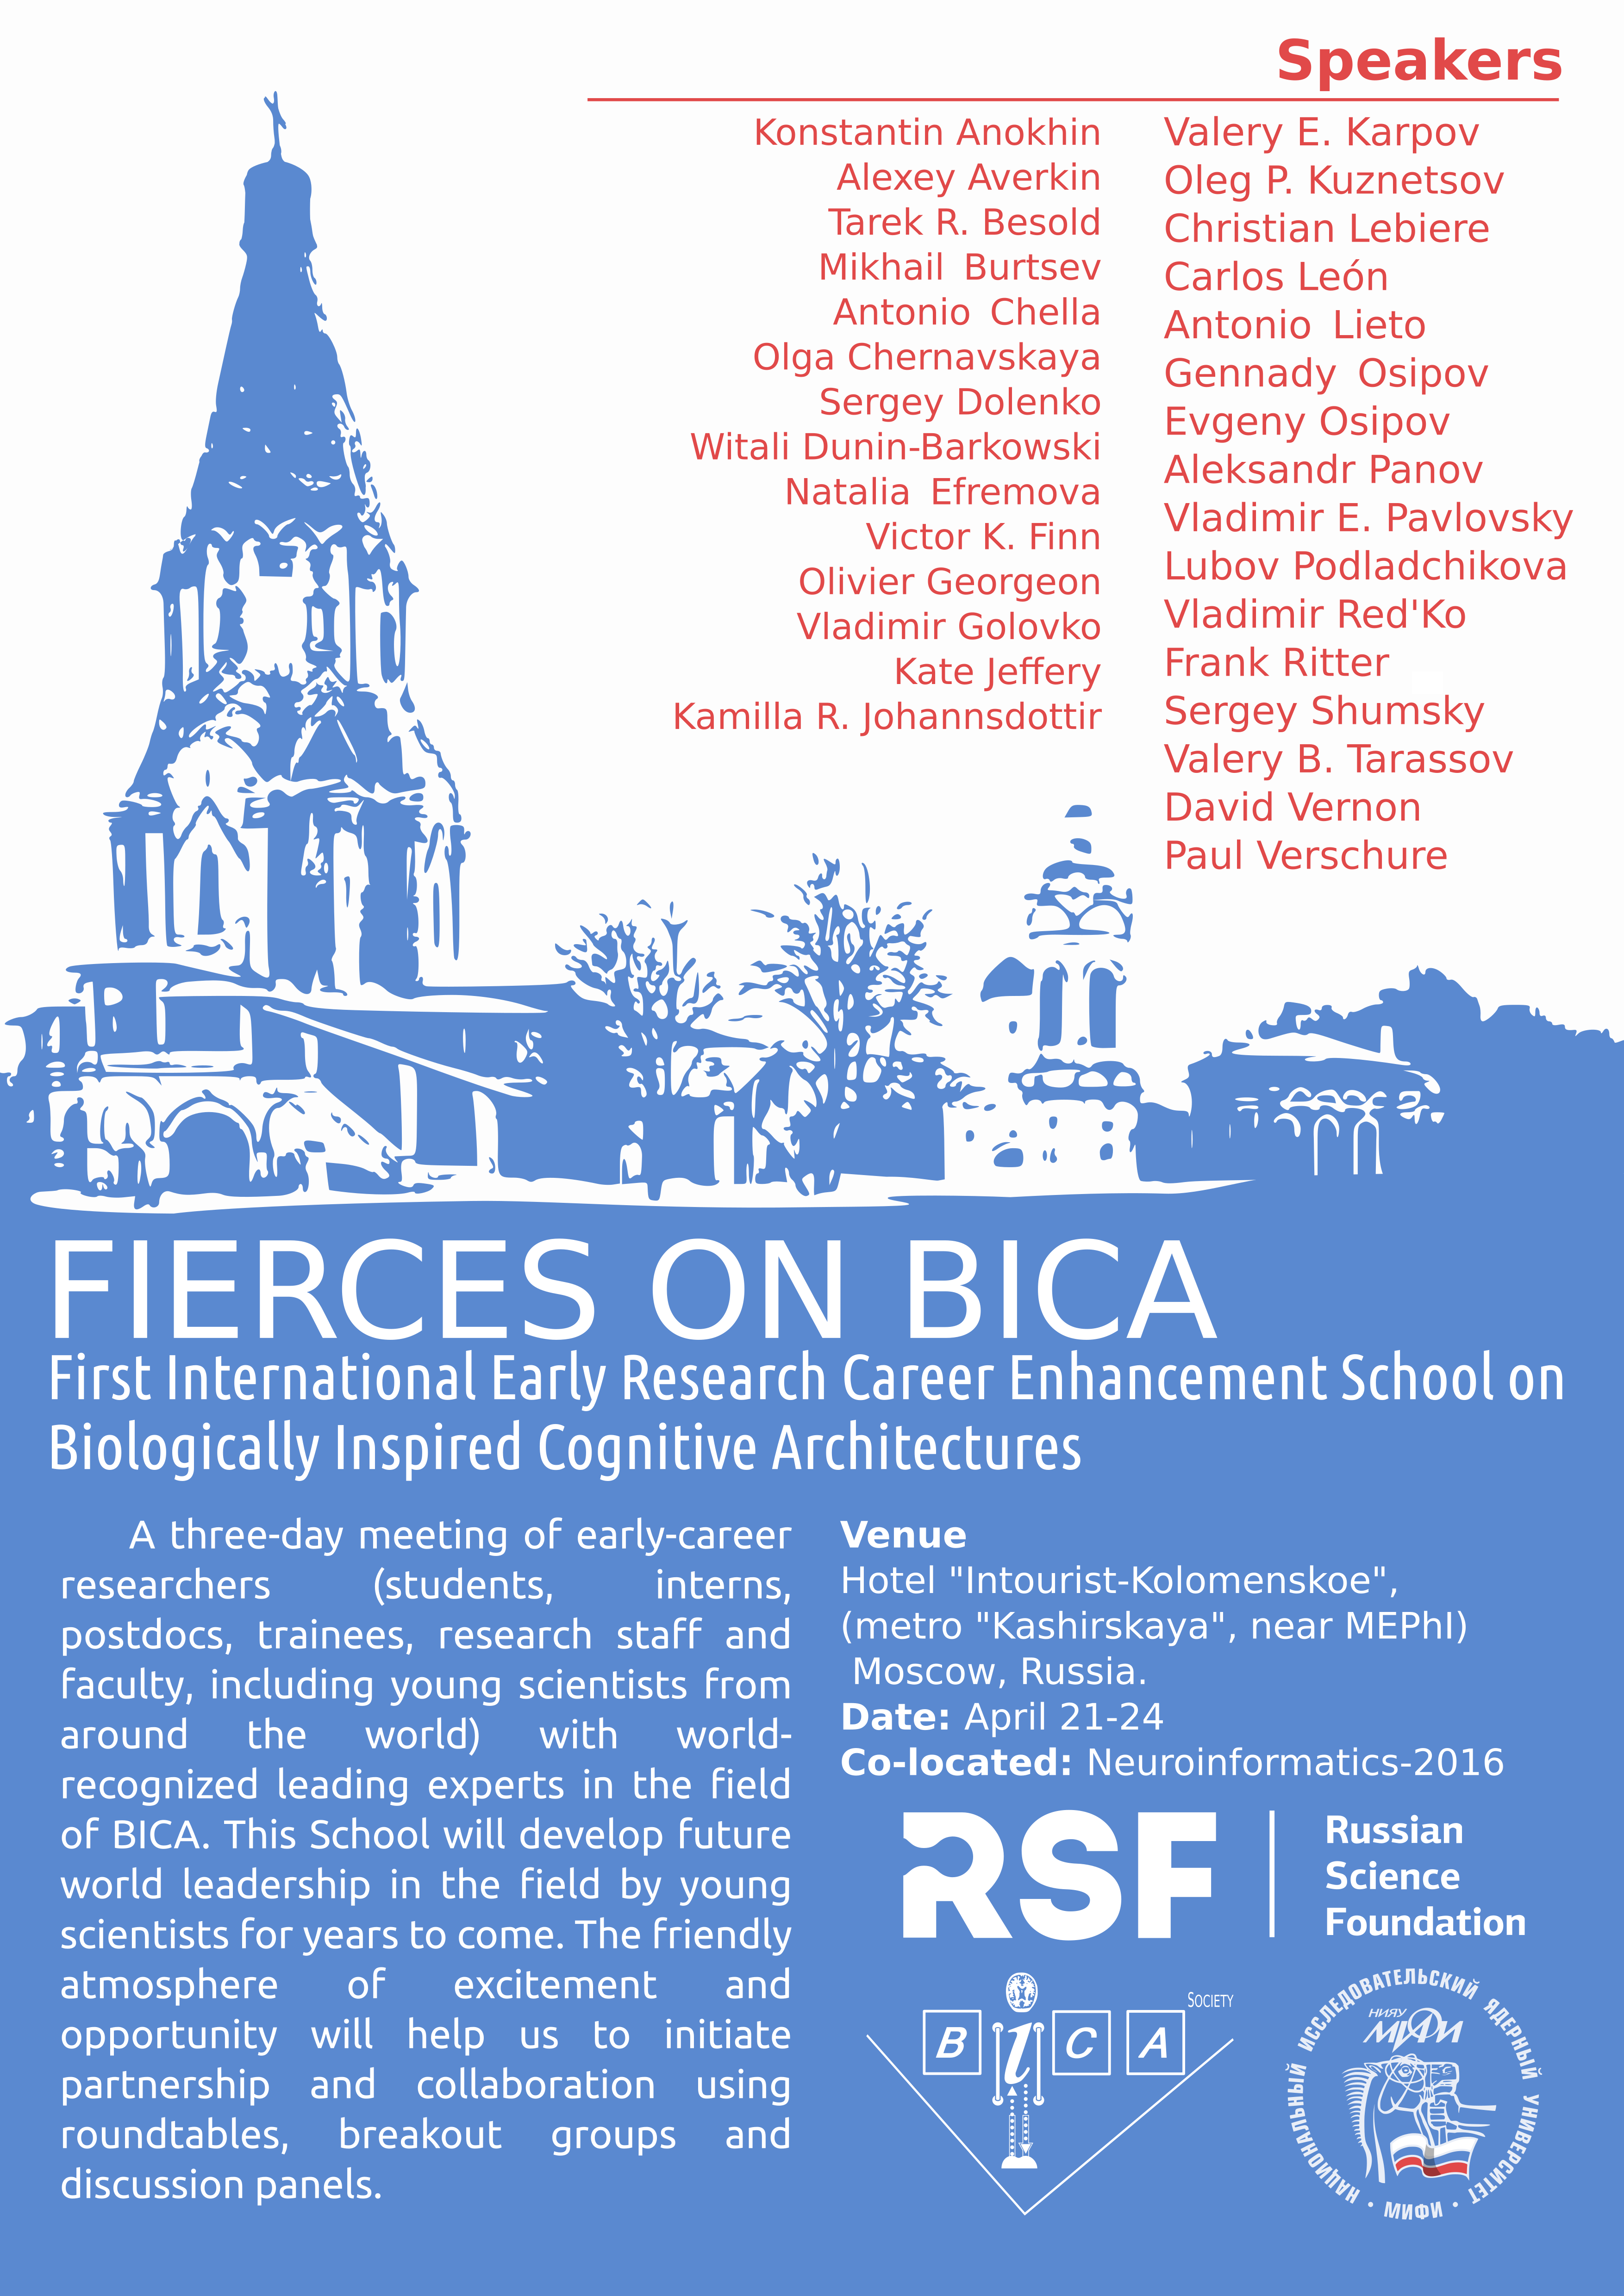
\includegraphics[width=\paperwidth]{title_back.png}}; % Background image
	\end{tikzpicture}};
\end{tikzpicture}
\vfill
\endgroup

%----------------------------------------------------------------------------------------

\end{document}